\documentclass[10pt,preprint,numbers]{sigplanconf}

\usepackage{amssymb}
\usepackage{amsmath}
\usepackage{amsthm}
\usepackage{stmaryrd}
\usepackage{color}
\usepackage{graphics}
\usepackage{fancyvrb}
\usepackage{subfigure}
\usepackage{multirow}
\usepackage{minted}
\usepackage{breqn}
\usepackage{enumitem}
%\usepackage{subcaption}
\usepackage{siunitx} % For pretty-printing numeric values and SI units
                     % of measure. e.g., the tabular column type S is
                     % used to print nice-looking tables of numbers.
\sisetup{ % defaults
  group-separator={,},
  group-minimum-digits={3},
  output-decimal-marker={.},
  table-format = 6
}

\usepackage{tikz}
\usepackage{xypic}
\usepackage{natbib}

\usetikzlibrary{calc}

%% http://tex.stackexchange.com/questions/55068/is-there-a-tikz-equivalent-to-the-pstricks-ncbar-command
\tikzset{
    ncbar angle/.initial=90,
    ncbar/.style={
        to path=(\tikztostart)
        -- ($(\tikztostart)!#1!\pgfkeysvalueof{/tikz/ncbar angle}:(\tikztotarget)$)
        -- ($(\tikztotarget)!($(\tikztostart)!#1!\pgfkeysvalueof{/tikz/ncbar angle}:(\tikztotarget)$)!\pgfkeysvalueof{/tikz/ncbar angle}:(\tikztostart)$)
        -- (\tikztotarget)
    },
    ncbar/.default=0.5cm,
}

\tikzset{round left paren/.style={ncbar=0.4cm,out=110,in=-110}}
\tikzset{round right paren/.style={ncbar=0.4cm,out=70,in=-70}}


\fvset{
  linenos=true,
  fontsize=\footnotesize,
  breaklines=true,
 breakafter=w),
  xleftmargin=\parindent,
  numbersep=1em
}

\usemintedstyle{vs}

\definecolor{darkblue}{rgb}{0.0,0.0,0.5}
\definecolor{darkgreen}{rgb}{0.0,0.4,0.0}
\definecolor{darkdarkgreen}{rgb}{0.0,0.35,0.0}

\usepackage{hyperref}
\hypersetup{
    unicode=false,          % non-Latin characters in Acrobat's bookmarks
    pdftoolbar=true,        % show Acrobat toolbar?
    pdfmenubar=true,        % show Acrobat menu?
    pdffitwindow=false,      % page fit to window when opened
    pdftitle={},    % title
    pdfauthor={}
    pdfsubject={},   % subject of the document
    pdfnewwindow=true,      % links in new window
    pdfkeywords={keywords}, % list of keywords
    colorlinks=true,       % false: boxed links; true: colored links
    linkcolor=darkblue,          % color of internal links
    citecolor=darkblue,        % color of links to bibliography
    filecolor=green,      % color of file links
    urlcolor=blue,          % color of external links
}

\usepackage{cleveref}
\crefname{section}{\S}{\S\S}
\Crefname{section}{\S}{\S\S}
\crefname{subsection}{\S}{\S\S\S}
\Crefname{subsection}{\S}{\S\S\S}
\crefname{figure}{fig.}{}
\Crefname{figure}{Fig.}{}
\crefname{definition}{def.}{}
\Crefname{definition}{Def.}{}

\CustomVerbatimEnvironment{SpecVerbatim}{Verbatim}{fontsize=\footnotesize,xleftmargin=0.5cm,
xrightmargin=0.2cm,commandchars=\\\{\},baselinestretch=0.98,numbersep=0.9em}
\CustomVerbatimEnvironment{ExmVerbatim}{Verbatim}{fontsize=\footnotesize,xleftmargin=0.5cm,
xrightmargin=0.2cm,baselinestretch=0.98,numbers=left,numbersep=0.9em,commandchars=\\\{\}}
\CustomVerbatimEnvironment{IVerbatim}{Verbatim}{fontsize=\relsize{-1},xleftmargin=0.5cm,
xrightmargin=0.2cm,commandchars=\\\{\},baselinestretch=0.98,numbersep=0.9em}


\definecolor{darkgreen}{rgb}{0.0,0.5,0.0}
\definecolor{darkpurple}{rgb}{0.6,0.0,0.6}
\definecolor{orange}{rgb}{0.8,0.4,0.0}
\definecolor{darkorange}{rgb}{0.5,0.2,0.0}
\definecolor{marco}{rgb}{0.0,0.3,0.5}
\definecolor{gray}{rgb}{0.2,0.2,0.2}

\newcommand\mdef{\stackrel{\mathclap{\normalfont\mbox{def}}}{=}}

\newcommand{\bn}{\mathbb{N}}

\newcommand{\todo}[1]{\textcolor{blue}{Dom: #1}}
\newcommand{\dnote}[1]{\textcolor{darkpurple}{Dom: #1}}
\newcommand{\mnote}[1]{\textcolor{darkgreen}{Mistral: #1}}
\newcommand{\anote}[1]{\textcolor{red}{Andy: #1}}

\newcounter{block}

\newtheorem{lemma}[block]{Lemma}
\newtheorem{proposition}[block]{Proposition}

\theoremstyle{definition}

\newtheorem{theorem}[block]{Theorem}
\newtheorem{remark}[block]{Remark}
\newtheorem{example}[block]{Example}
\newtheorem{definition}[block]{Definition}

% Writing macros
\newcommand{\ie}{\emph{i.e.}}
\newcommand{\eg}{\emph{e.g.}}

\newcommand{\dimId}{\texttt{dim}}

% Semantics related
\newcommand{\interp}[1]{\llbracket{#1}\rrbracket}

% Syntax macros
\newcommand{\nonterm}[1]{\textit{#1}}
\newcommand{\term}[1]{\texttt{#1}}

\newcommand{\stenRefl}[1]{\term{pointed} \, (\term{dim=}#1)}
\newcommand{\stenFwd}[3]{\term{forward} \, (\term{depth=}#1,
  \term{dim=}#2{#3})}
\newcommand{\stenBwd}[3]{\term{backward} \, (\term{depth=}#1,
  \term{dim=}#2{#3})}
\newcommand{\stenCen}[3]{\term{centered} \, (\term{depth=}#1,
  \term{dim=}#2{#3})}
\newcommand{\irrefl}{\texttt{nonpointed}}

\newcommand{\stenReflS}[1]{\term{pointed} \, (\term{dim=}#1)}
\newcommand{\stenFwdS}[2]{\term{fwd} \, (\term{depth=}#1,
  \term{dim=}#2)}
\newcommand{\stenBwdS}[2]{\term{bwd} \, (\term{depth=}#1,
  \term{dim=}#2)}
\newcommand{\stenCenS}[2]{\term{cen} \, (\term{depth=}#1,
  \term{dim=}#2)}
\newcommand{\irreflS}{\texttt{np}}

\newcommand{\stenFwdSR}[3]{\term{fwd} (\term{depth=}#1,
  \term{dim=}#2, #3)}
\newcommand{\stenBwdSR}[3]{\term{bwd} (\term{depth=}#1,
  \term{dim=}#2, #3)}
\newcommand{\stenCenSR}[3]{\term{cen} (\term{depth=}#1,
  \term{dim=}#2, #3)}
\newcommand{\stenReflSR}[1]{\term{point} (\term{dim=}#1)}

% SYNTAX OPERATIONS AND PREDICATES
%\newcommand{\neigh}{\textsf{neigh}}
\newcommand{\arrayTy}{\textsf{array}}
\newcommand{\rhsExp}{\textsf{rhsExp}}
\newcommand{\var}{\textsf{var}}

%% VECTOR NOTATIONS
\newcommand{\vect}[1]{\textbf{#1}}

\newcommand{\vtwohs}[2]{\setlength{\arraycolsep}{0em}
\left[\begin{array}{cc}#1 \, & \, #2\end{array}\right]\!}

\newcommand{\vtwoh}[2]{\setlength{\arraycolsep}{0em}
\left[\begin{array}{cc}#1 \; & \; #2\end{array}\right]}

\newcommand{\vthreeh}[3]{\setlength{\arraycolsep}{0em}
\left[\begin{array}{ccc}#1 \; & \; #2 \; & \; #3\end{array}\right]}
\newcommand{\vtwo}[2]{\setlength{\arraycolsep}{0em}
\left[\begin{array}{l}#1\\#2\end{array}\right]}
\newcommand{\vthree}[3]{\setlength{\arraycolsep}{0em}
\left[\begin{array}{l}$#1$\\$#2$\\$#3$\end{array}\right]}
\newcommand{\stwo}[4]
%{\vtwo{#1}{#2}\!\vtwo{#3}{#4}}
{\setlength{\arraycolsep}{0.1em}
\left[\begin{array}{rr}$#1$ & $#3$\\$#2$ & $#4$\end{array}\right]}

\newcommand{\singleEntry}[2]{\textbf{J}_{#2}^{#1}}
\newcommand{\zeroEntry}[2]{\textbf{K}_{#2}^{#1}}

%% OPERATIONS ON SPANS and VECTORS
\newcommand{\containedin}{\sqsubseteq}

%% MODEL
\newcommand{\effdims}[2]{\mathit{constr}(#1)_{#2}}

\newcommand{\trule}[1]{{\footnotesize{(\text{#1})}}}
%\include{results}


%\newcommand{\cons}[3]{\mathbf{C}_{#3}(#1, #2)}
\newcommand{\consName}{\textbf{agree\textprime}}
\newcommand{\cons}[2]{#1 \,\, \consName{} \,\, #2}
\newcommand{\consAName}{\textbf{agree}}
\newcommand{\consA}[2]{#1 \,\, \consAName{} \,\, #2}
\newcommand{\consSub}[3]{#2 \,\, \consAName{}_{#1} \,\,#3}


\title{Verifying Spatial Properties of Stencil Computations}
%\titlebanner{DRAFT -- Do not distribute}
\authorinfo{}{}{}
%\preprintfooter{DO NOT DISTRIBUTE}


\begin{document}
\maketitle

\bibliographystyle{plain}

\begin{abstract}
Stencil computations are a common programming pattern in numerical
  code and typically form the core of graphics and scientific
  computing applications. However, they are often complex and
  unwieldy, involving substantial fine-grained manipulation of array
  indices across multiple arrays and dimensions. This requires careful
  testing, which is almost always done manually and then discarded
  during development. In this paper, we propose an alternate approach:
  a specification language and automated tool for verifying the
  spatial behaviour of stencils. The specification language is based
  on the hypothesis that stencil computations read from arrays with a
  regular, fixed pattern which can be captured abstractly by a simple
  set of combinators in our specification language. These
  specifications can be embedded as annotations in source code,
  against which code can be checked for conformance. For legacy code,
  spatial specifications can be inferred, providing documentation and
  aiding future software maintenance. We evaluate our language against
  a corpus of numerical Fortran code, and show that the vast majority
  of stencil computations indeed have a simple, regular, static shape
  validating the design of our language.  We introduce the
  language, checking and inference procedures, and its evaluation.
\end{abstract}

%\keywords{program verification, specification, stencils}


\section{Introduction}\label{sec:intro}

\emph{Stencils} are a ubiquitous programming pattern, common in
scientific and numerical computing applications. Informally, a stencil
computation computes an array whose value at each index $i$ is
calculated from a \emph{neighbourhood} of values around $i$ in some
input array(s), \eg{}, the Game of Life, convolutions in image
processing, approximations to differential equations. For example, the
following computes the one-dimensional discrete Laplace transform (an
approximation to a derivative) in Fortran:
%
\begin{minted}{fortran}
do i = 1, (n-1)
      b(i) = a(i-1) - 2*a(i) + a(i+1)
end do
\end{minted}
%
Values \texttt{b(i)} are calculated from a neighbourhood of elements
around \texttt{i} in the input array \texttt{a}.  In this example, the
access pattern is simple and easily understood. More complex
stencil computations are more prone to errors from simple lexical
mistakes. For example, the following is a small snippet from a
Navier-Stokes fluid simulator (based on~\citet{griebel1997numerical})
 in which two arrays are read with
different data access patterns, across two dimensions.
%%
\begin{minted}[firstnumber=20,xleftmargin=2em]{fortran}
du2dx = ((u(i,j)+u(i+1,j))*(u(i,j)+u(i+1,j))+   &
  gamma*abs(u(i,j)+u(i+1,j))*(u(i,j)-u(i+1,j))- &
  (u(i-1,j)+u(i,j))*(u(i-1,j)+u(i,j))-          &
  gamma*abs(u(i-1,j)+u(i,j))*(u(i-1,j)-u(i,j))) &
  /(4.0*delx)

duvdy = ((v(i,j)+v(i+1,j))*(u(i,j)+u(i,j+1))+   &
  gamma*abs(v(i,j)+v(i+1,j))*(u(i,j)-u(i,j+1))- &
  (v(i,j-1)+v(i+1,j-1))*(u(i,j-1)+u(i,j))-      &
  gamma*abs(v(i,j-1)+v(i+1,j-1))*(u(i,j-1)-     &
  u(i,j))) / (4.0*dely)

laplu = (u(i+1,j)-2.0*u(i,j)+u(i-1,j))/delx/delx+ &
  (u(i,j+1)-2.0*u(i,j)+u(i,j-1))/dely/dely

f(i,j) = u(i,j)+del_t*(laplu/Re-du2dx-duvdy)
\end{minted}
%%
The access pattern is much harder to understand than the
one-dimensional Laplace.  The miasma of indexing expressions of the
form \texttt{var(i$\pm$a, j$\pm$b)} is not only hard to read, but is
prone to simple textual input mistakes, \eg{}, swapping \texttt{-} and
\texttt{+}, missing an indexing term, or transforming the wrong
variable \eg{} \texttt{(i+1,j)} instead of \texttt{(i,j+1)}.

In practice, the typical development procedure for complex
stencil computations involves some ad hoc testing to ensure that no
transcription mistakes have been made (\eg{}, by visual
inspections, or comparison against an manufactured or 
analytical solutionst~\cite{farrell2010automated}). Typically such
testing is discarded once the code is seen to be correct.

This is not the only information that is often discarded. The
``shape'' of the indexing pattern is usually the result of choices made in the
numerical-analysis procedure to convert some
continuous equations into a discrete approximation. Rarely are these
decisions captured in the source code, yet the shape of access is
usually uniform and is has a perspicuous and concise description in
numerical analysis literature \eg{}, ``\emph{centered in space, to a
  depth of 1}'' referring to indexing terms \texttt{a(i)},
\texttt{a(i-1)} and \texttt{a(i+1)}.

To support the development of correct stencil computations, we propose
a simple, abstract specification language for the data access pattern
of stencils. The shape of the
Laplace example stencil is specifed in our language as:
%
\begin{minted}[linenos=false]{fortran}
!=  stencil centered(depth=1, dim=1) :: a
\end{minted}
%
This describes \texttt{a} is accessed with a symmetrical pattern
(``centered'') to a depth of one in each direction in its first
dimension.  The shape of the Navier-Stokes example
is specified as:
%
\begin{minted}[linenos=false,xleftmargin=0em,xrightmargin=0.8em,breakindent=1.9em]{fortran}
!= stencil centered(depth=1,dim=1)*pointed(dim=2)     + centered(depth=1,dim=2)*pointed(dim=1) :: u

!= stencil forward(depth=1,dim=1)                          * backward(depth=1,dim=2) :: v
\end{minted}
%
The specification requires that, over the whole fragment, \texttt{u}
is accessed with a centered pattern to depth of 1 in both dimensions
(this is known as the \emph{five-point stencil}) and \texttt{v} is
accessed in a neighbourhood bounded forwards to depth of $1$ in the
first dimension and backward to a depth of $1$ in the second
dimension. Note the relatively small size of the specification
compared to the source code, and its high-level of abstraction.

We provide a verification tool which can check the spatial correctness
of stencil computations against a specification. Furthermore, the tool
can automatically infer specifications and insert these as comments
into the source code. The main features and benefits of our approach
are as follows:
%
\begin{itemize}
%\item The main use case is that a programmer writes a specification
%  first (perhaps informed by their numerical analysis), then writes
%  the corresponding source code, and lastly has the tool check its
%  conformance to the specifications. This specify-and-check approach
%  removes the usually ad hoc testing effort, and provides the
%  opportunity for easy re-verification in the event of any refactoring
%  of software maintenance activities.
\item The primary use case is that a programmer writes a specification first,
  then writes the corresponding source code. Our tool then checks conformance between
  the two. This specify-and-check approach reduces testing effort and
  future-proofs against bugs introduced during refactoring and maintanence.
%
%\item The specification provides a concise description which can be
%  preserved in the source code to provide documentation to future
%  developers, contrasting with ad hoc tests which are usually
%  discarded or specialised to the development environment. Separate from the
%  verification procedure, the infer-and-synthesise mode of the tool
%  provides a way to automatically generate additional useful
%  documentation for future users.

% Emphasis here is on documentation generation, so it makes little sense to
% compare this aspect of CamFort to ad hoc testing. Apples and oranges.
\item A specification concisely captures the access pattern of a
  stencil and turns it into documentation. The inference procedure
  efficiently produces specifications with no programmer intervention,
  automatically inserting specifications at appropriate places in the
  source code.
%
%\item Specifications are integrated into the code as comments for easy
%  integration with existing tools, as well as documentation systems (\eg{}, we
%  support Doxygen and FORD syntax).
%
\item Our specification format is deliberately abstract, with a small number of
  combinators that \emph{do not involve any indexing expressions}, \eg{}
  \texttt{a(i+1,j-1)}. This contrasts with other specification approaches. If a
  user specifies, say, the Naiver-Stokes stencil above, in a deductive
  verification language such as ACSL, they must write a specification involving
  textually dense array-indexing expressions. Therefore, any low-level mistakes
  that could be made whilst programming complex indexing code could also be
  made when writing its specification. Our specifications are more lightweight
  with the aim of aiding adoption by scientists and preventing indexing errors.
\end{itemize}

Our verification tool does not target a
class of bugs that can be detected automatically (\emph{push-button
  verification}). Instead, stencil computation bugs must be
identified relative to a specification of the intended access pattern.

In this paper, we make the following contributions:
%
\begin{itemize}
\item We introduce a specification language for stencils
  that captures common forms of data access patterns
  (\cref{sec:lang});

\item We detail checking and inference algorithms for our
  specifications (\cref{sec:analysis}), derived from a
  denotational model for the specificaiton language
  (\cref{sec:semantics});

\item We provide an implementation of our approach as an extension to
  CamFort, an open-source program analysis tool for Fortran;

\item We report on a quantitative study of stencil computations on a
  corpus of numerical Fortran program
  (\cref{sec:evaluation}), totalling one million lines of code. Our tool
  identifies and infers specifications for 35,000 stencil computations in the
  corpus. Approximately 10\% of the stencils we found are non-trivial,
  corresponding to code which is a possible source of errors. This validates
  our hypothesis that the majority of stencil computations have a regular
  shape, and validates the design of our language in its capability to capture
  many core patterns.

\item We give a detailed verification case study of two
  stencil computations commonly used in scientifc computing,
  simulating programming errors. Our approach detects all
  possible indexing errors for these computations.
\end{itemize}
%

\newcommand{\domainVal}{\mathbb{Z}_\infty}
\section{Stencil specifications}\label{sec:lang}

Our specification language is based on the hypothesis
that most forms of array access in numerical code have
a fixed, statically-determined access pattern. For example, the
\emph{five-point stencil} on a two-dimensional array reads from array
indices $(i, j)$, $(i-1, j)$, $(i+1, j)$, $(i, j-1)$, and $(i, j+1)$
for all $i, j$ within the inner boundary of the array (to avoid
out-of-bounds access at the edges). We revisit this hypothesis
in \cref{sec:evaluation} with the inference of
such regular stencil patterns on our corpus of numerical programs.

We give various definitions used in the paper then
\cref{subsec:syntax} outlines the syntax of stencil specifications
with an informal introduction. \cref{sec:semantics}
gives a semantic model via a set-based interpretation which makes
concrete the meaning of specifications. \cref{sec:eqs} then provides
a syntactic equational theory for specifications which is
sound with respect to the model.
%sub-specification for which the
%equality and sub-specification relation are proven sound.


\paragraph{Notation}
%\label{sec:notation}

\renewcommand*{\arraystretch}{0.8}
For the target language, $e$ ranges over expressions (may be impure) and $v$
over its (imperative) variables. %By
%``variable'', we mean in the imperative sense (named binders to memory cells).

\begin{definition}[Induction variable]
  An integer variable is an \emph{induction variable} if it is the control
  variable of a ``\texttt{for}'' loop incremented by $1$ per iteration. A variable
  is interpreted as an induction variable only within the scope of the loop
  body. Throuhgout, $i, j, k$ range over induction variables.
%TODO: consider mentioning derived, non-based induction variables
% as we did before.
\end{definition}

\begin{definition}[Array subscripts and indices]
  An \emph{array subscript}, denoted $a(\bar{e})$, is an expression
  which reads from an array $a$ at an \emph{index} specified by a
  comma-separated sequence of integer expressions denoted $\bar{e}$ or
  in expanded form as $(e_1, \ldots, e_n)$. An index $e_i$
  is called \emph{relative} if the expression involves an induction
  variable.
  An \emph{absolute index} is a constant integer expression relative to the
  enclosing loop.
\end{definition}

\begin{definition}[Neighbourhood index]
\label{def:neighbour}
  For an array subscript $a(\bar{e})$ an index $e \in \bar{e}$ is a
  \emph{neighbourhood index} if $e$ is of the form $e \equiv i$, $e \equiv i +
  c$, or $e \equiv i - c$, where $c$ is an integer constant. That is, a
  neighbourhood index is a constant translation of an induction variable. (The
  relation $\equiv$ identifies terms up-to commutativity of $+$ and the inverse
  relationship of $+$ and $-$ \eg{}, $(-b) + i \equiv i - b$).
\end{definition}

\begin{definition}[Stencil computations]
\label{def:stencil}
  Let $a$ be an array of dimensionality $n$ and $\overline{b}$ a
  collection of arrays of arbitrary (possibly differing)
  dimensionalities.
  A \emph{stencil computation} comprises an iteration by a set $I$ of at
  most $n$ induction variables
  over a subset of the index space of $a$. Each iteration
  determines the elements of $a$ by an
  assignment $a(\bar{e}) = e_r$ where each $e \in
  \bar{e}$ is either a neighbourhood or constant index.
  For all $b \in \bar{b}$ and array subscripts $b(\bar{e}')$
  that flow to $e_r$, each $e' \in \bar{e}'$ is
  either a neighbourhood or absolute index.

  We refer to the assignment $a(\bar{e}) = e_r$ and all the associated
  statements with dataflow to $e_r$ as the \emph{stencil kernel}.
\end{definition}
%
% specifying the shape of indexing expressions for
%arrays $\bar{v}$ that are simultaenously permitted and expected within
%the code to which the specification is given.
%
%\marginpar{\dnote{Is it worth having this informal consistency here?}}

For now we informally describe what it means for a stencil kernel to
be consistent with a specification. This will be formalised in
\Cref{sec:semantics} and algorithmically described in and
\Cref{sec:analysis}.  Specifications are associated to a stencil
kernel and are declared for one or more array variables $\bar{v}$
within that kernel.  A stencil specification defines a \emph{region}
associated to an array variable $a$ against which a stencil kernel
should be \emph{consistent}. The region defined by a specification is
an $n$-dimensional rectilinear shape in a discrete space crossing the
origin with respect to the induction variable. Consistency is then a
two way requirement. All array subscripts on $a$ contributing to the
kernel should be consistent with the region. Conversely, all parts of
the region should have an index corresponding it.

\begin{figure}[t]
\vspace{-0.9em}
\begin{align*}
\def\arraystretch{1}
\setlength{\arraycolsep}{0.2em}
\newcommand{\dimTy}{\mathbb{N}_{>0}}
\begin{array}{rl}
\nonterm{specification} ::= & \nonterm{regionDec} \mid \nonterm{specDec} \\
\nonterm{specDec} ::= & \term{stencil} \; \nonterm{spec} \;
                        \texttt{::} \; v \\
\nonterm{regionDec} ::= &  \texttt{region} \; \texttt{::} \; \nonterm{rvar} \; \texttt{=} \;
                         \nonterm{region}\\[0.4em]
%\nonterm{spec} ::= & \nonterm{spatial} \mid \nonterm{temporal}
%\\[1em]
\nonterm{spec} ::= & [\nonterm{mult},] \; [\nonterm{approx},] \; \nonterm{region} \\
\nonterm{mult} ::= & \term{readOnce} \\
\nonterm{approx} ::= & \term{atMost} \; \mid \; \term{atLeast} \\[0.1em]
\nonterm{region} ::= & \nonterm{rvar} \; \\
\multicolumn{2}{l}{\qquad \mid \; \stenRefl{\dimTy}} \\
\multicolumn{2}{l}{\qquad \mid \;\stenFwd{\mathbb{N}_{>0}}{\dimTy}{\;[, \texttt{nonpointed}]}} \\
\multicolumn{2}{l}{\qquad \mid \; \stenBwd{\mathbb{N}_{>0}}{\dimTy}{\;[, \texttt{nonpointed}]}} \\
\multicolumn{2}{l}{\qquad \mid \; \stenCen{\mathbb{N}_{>0}}{\dimTy}{\;[, \texttt{nonpointed}]}} \\
\multicolumn{2}{l}{\qquad \mid \; \nonterm{region} \, \term{+}
  \, \nonterm{region} \; \mid \; \nonterm{region} \; \term{*} \; \nonterm{region}} \\[0.25em]
%\multicolumn{2}{l}{\qquad\qquad \mid \; \nonterm{rvar}}
%\\[0.5em]
%\nonterm{temporal} ::= \; & \term{dependency} \; (v \; \{ , v \}) [, \texttt{mutual}]
%  \\[0.5em]
\nonterm{rvar} ::= \; & [\text{\term{a}-\term{z}$\,$\term{A}-\term{Z}$\,$\term{0}-\term{9}}]+\\[-1em]
\end{array}
\end{align*}
\caption{Specification syntax (EBNF grammar)}
\label{fig:syntax}
\vspace{-0.8em}
\end{figure}


\subsection{Specification syntax}
\label{subsec:syntax}

\Cref{fig:syntax} gives the syntax of stencil specifications, which is
detailed below. The entry point is the \nonterm{specification} production which
splits into either a \emph{region declaration} or a \emph{specification
declaration}.
Regions comprise \emph{region constants} which are
combined via region operators \term{+} and \term{*}.

\paragraph{Region constants}

Region constants specify a finite contiguous region in a
single dimension relative to the origin and are either \term{pointed},
\term{forward}, \term{backward}, or \term{centered}.  Each region
constant has a dimension identifier $d$ given as a positive natural number.
Each constant except \term{pointed} has a depth
parameter $n$ given as a positive natural number; \term{pointed}
regions implicitly have a depth of $0$.

A \term{forward} region of depth $n$ specifies a continguous
region in dimension $d$ starting at the origin. This corresponds
to specifying neighbourhood indices in dimension $d$ ranging from $i$ to $i + n$
for some induction variable $i$. Similarly, a
\term{backward} region of depth $n$ corresponds to contiguous indices
from $i$ to $i - n$ and \term{centered}
of depth $n$ from $i - n$ to $i + n$. A \term{pointed}
stencil specifies a neighbour index $i$. For example, the
following shows four specifications with four consistent stencil
kernels reading from arrays \term{a}, \term{b}, \term{c} and \term{d}:
%%
\begin{minted}{fortran}
!= stencil forward(depth=2, dim=1) :: a
e(i, 0) = a(i, 0) + a(i+1, 0) + a(i+2, 0)
!= stencil backward(depth=2, dim=1) :: b
e(i, j) = b(i, j) + b(i-1, j) + b(i-2, j)
!= stencil centered(depth=1, dim=2) :: c
e(i, j) = (c(j-1) + c(j) + c(j+1))/3.0
!= stencil pointed(dim=3) :: d
e(i, j) = d(0, 0, i)
\end{minted}
%%
Not every dimension needs to be specified, \eg{},
specifications on lines $1$, $3$, and $7$ leave some dimensions unspecified.

The \term{forward}, \term{backward}, and \term{centered} regions may
all have an additional attribute \term{nonpointed} which marks absence
of the origin.  For example, the following is a
\term{nonpointed} \term{backward} stencil
%
\begin{minted}{fortran}
!= stencil backward(depth=2, dim=1, nonpointed) :: a
b(i) = a(i-1) + 10*a(i-2)
\end{minted}

\paragraph{Combining regions}

% r+s means that indices must be consistent with either r or s
% r*s means that indices must be consistent with both r and s at the
% same time

% specifications correspond to a set of schemes

% r+s means an index must be generalised by a scheme in either r or s
%       and every scheme in r must have an index which specialises it
%       and every scheme in s must have an index which specialises it

% r*s means an index must be generalised by a scheme in r and a scheme in s
%       and every pairs of schemes in r and s must have an index which
%           specialises both
%

The region operators \term{+} and \term{*} respectively combine
regions disjunctively and conjuctively.

The conjuction of two regions $r \term{*} s$ means that any indices
in the specified code must be consistent with both $r$ and $s$
simultaenously. Dually, for every pair of components in the regions
$r$ and $s$ there must be an index consistent with both.
For example, the following \emph{nine-point stencil}
has a specification given by the product of two \texttt{centered}
regions in each dimension:
%%
\begin{minted}[breakindent=2.9em]{fortran}
x = a(i, j)   + a(i-1, j)   + a(i+1, j)
y = a(i, j-1) + a(i-1, j-1) + a(i+1, j-1)
z = a(i, j+1) + a(i-1, j+1) + a(i+1, j+1)
!= stencil centered(depth=1, dim=1) * centered(depth=1, dim=2) :: a
b(i, j) = (x + y + z) / 9.0
\end{minted}
%%
This pattern is common in image convolution applications.
The specification ranges over the
values that flow to the array subscript on the left-hand side,
and so ranges over the intermediate assignments to \term{x},
\term{y}, and \term{z}. Each index in the code is consistent
with both specifications simultaneously, \eg{}, \texttt{a(i-1, j+1)}
is within the centered region in dimension $1$ and the centered region
in dimension $2$.

The product $r \term{*} s$ can also be thought of as a bounding box
over the two regions $r$ and $s$.

The disjunction of two regions $r \term{+} s$ means that any indices
in the spcified code must be consistent with either of $r$ or $s$.
Dually, every part of region $r$ must have a
corresponding index and similarly for $s$ independently. For
example, the following gives the specification of a five-point
stencil which is the sum of two compound \texttt{pointed} and
\texttt{centered} regions in each dimension:
%
\begin{minted}{fortran}
!= stencil centered(depth=1, dim=1)*pointed(dim=2)    + centered(depth=1, dim=2)*pointed(dim=1) :: a
b(i,j) = -4*a(i,j) + a(i-1,j) + a(i+1,j) &
                   + a(i,j-1) + a(i,j+1)
\end{minted}
%%
Here the left-hand side of \texttt{+} says that when the second dimension
(induction variable $j$) is fixed at the origin, the first dimension
(induction variable $i$) accesses the immediate vicinity of the origin
(to depth of one). The right hand side of \texttt{+} is similar but the dimensions are reversed.
This reflects the symmetry under rotation of the five-point stencil.

\paragraph{Region declarations and variables}

Region specifications can be assigned to region variables via
region declarations. For example, the shape of a
``\emph{Roberts cross}'' edge-detection convolution~\cite{davis1975survey}
can be stated:
%%
\begin{minted}{fortran}
!= region :: r1 = forward(depth=1, dim=1)
!= region :: r2 = forward(depth=1, dim=2)
!= region :: robertsCross = r1*r2
!= stencil robertsCross :: a
\end{minted}
This is useful for common stencil patterns, such as the five-point
pattern, as the region can be defined once and reused.
%%
\paragraph{Modifiers}
%%
Region specifications can be modified
by \emph{approximation} and \emph{multiplicity} information
(in \textit{spec} in \Cref{fig:syntax}).

The \texttt{readOnce} modifier enforces that no index appears more
than once (that is, its multiplicity is one). For example, all of
the previous examples could have \texttt{readOnce} added:
%
\begin{minted}{fortran}
!= stencil readOnce, backward(depth=2, dim=1) :: a
b(i+1) = a(i) + a(i-1) + a(i-2)
\end{minted}
%
This specification would be invalid if any of the
array subscripts were repeated. This modifier provides a way to
rule out any accidental repetition of array subscripts.
The notion is similar to that of \emph{linearity} in linear type
systems~\cite{wadler1990linear}, where a value must be used
exactly once. We opt for the more informative and easily understood name
\texttt{readOnce}. This modifier is optional, so it need not
be present even if the stencil is linear.

In some cases, it is useful to give a lower and/or upper bound for a
stencil. This can be done using either the \term{atMost} or
\term{atLeast} modifiers. This is particularly useful in situations
where there is a non-contiguous stencil pattern, which cannot be expressed
precisely in our syntax. For example:
%
\begin{minted}{fortran}
!= stencil atLeast, pointed(dim=1)         :: a
!= stencil atMost, forward(depth=4, dim=1) :: a
b(i) = a(i) + a(i+4)
\end{minted}

\section{A model for specifications}
\label{sec:semantics}

We define a simple set-theoretic denotational model of the semantics
of our specification language. This has a number of purposes:
(1) it serves to explain the meaning of our specifications
(2) it is used in the inference and checking algorithms
(\Cref{sec:analysis}); (3) justifies an equational theory for
specifications in the next section; and (4) can be used to guide
correct implementations. The model domain is over sets of vectors
which we call \emph{index schemes}.

\begin{definition}
  An \emph{index scheme} is a vector of size $n$ (an $n$-vector) with
  values drawn from $\domainVal = \mathbb{Z} \cup \{\infty\}$.  Values
  in $\mathbb{Z}$ represent the offsets of neighbourhood indices
  (\ie{}, the constant integer $c$ in an indexing expression of the
  form $i \pm c$, \Cref{def:neighbour}) and $\infty$ is a wild-card
  representing both constant indices and unspecified indices.
  For an index scheme $u$, the $i^{th}$ element is denoted $u_i$. We
  write $(\domainVal)^n$ for the set of all $n$-dimensional schemes.
\end{definition}

Indexing schemes abstract array subscripts.
Our model represents the meaning of stencil specifications
as indexing schemes, which explain the range of possible
indexing behaviours which are consistent with the specification.
The relationship between source language
terms and index schemes
 is given precisely by the following function \textsf{schematic},
 which forms part of checking and inference (\Cref{sec:analysis}).

\newcommand{\schemeOne}{\textsf{s}_I}
%\newcommand{\schemeOne}{\textsf{schema$^1_I$}}
\newcommand{\schemeN}{\textsf{schematic}_I}
%\newcommand{\schemeN}{\textsf{schema$^n_I$}}
\begin{definition}%[Schematic]
\label{def:schematic}
Let $\schemeOne$ be a partial function, parameterised by a set of
induction variables $I$, mapping source langauge expressions to
$\domainVal$ values:
%%
\begin{align*}
\schemeOne(e)
 & =  \begin{cases}
c & e \equiv i + c \;\; \wedge \;\; i \in I \\
-c & e \equiv i - c \;\; \wedge \;\; i \in I \\
\infty & \textit{$I \cap \textit{FreeVariables}(e) = \emptyset $} %\\
%\bot   & \textit{otherwise}
\end{cases}
\end{align*}
In the
first two cases, expressions that are a constant offset of an
induction variable (\ie{}, neighbourhood indices) are mapped to the
offset $c$ or $-c$ $\in \domainVal$. In the third case, if the
expression is not defined in terms of an induction variable, it
is mapped to $\infty \in \domainVal{}$. Otherwise, $\schemeOne(e)$
is undefined ($\bot$).

The partial function $\schemeN$, also parameterised by a set of
induction variables $I$, uses $\schemeOne$ to
 map from the syntax of indices to index schemes
$\in (\domainVal)^n$. It is defined on the syntax of indices $\bar{e} = (e_1, ..., e_n)$ as:
\begin{align*}
\schemeN(e_1, .., e_n) & =
[\schemeOne(e_1) ... \schemeOne(e_n) ]
\; \textit{iff} \; \forall x . \schemeOne(e_x) \neq \bot
\end{align*}
%
Thus, if each expression in an index is a neighbourhood or constant
index, $\schemeN$ maps it to an indexing scheme.
\end{definition}

\begin{definition}[Generalisation]
\label{def:generalisation}
Given two schemes $v, w$ of dimensionality $n$,
then $w$ is said to \emph{generalise} $v$
(or conversely $v$ \emph{specialises} $w$),
written $v \preceq_n w$ defined:
\[
v \preceq_n w \;\; \Leftrightarrow  \;\;
  \forall i\!\in\!\{ 1, \ldots, n \} . \, (w_i = \infty \, \vee \, v_i = w_i)
\]
%%
where $\preceq_n$ is a reflexive, transitive relation on
index schemes $\domainVal^n$. Thus,
 $\infty$ generalises any index in the same dimension.
%
\end{definition}

\begin{example}
Consider the following array subscript to indexing schemes
conversions:
%
\begin{align*}
\begin{array}{ll}
\schemeN{(i, j+1)} & =\vtwoh{0}{1} \\
\schemeN{(1, j+1)} & = \vtwoh{\infty}{1} \\
\schemeN{(i*2, j)} & = \bot
\end{array}
\end{align*}
There is one generalisation between these
schemes, namely that $\vtwoh{0}{1} \preceq_2 \vtwoh{\infty}{1}$.
The last example is undefined as its first expression is a
non-neighbour relative index.
\end{example}

Our terminology of \emph{index schemes} and
\emph{generalisation} is by analogy
with the \emph{type schemes} and \emph{type generalisation} of
polymorphic types in ML~\cite{milner1978theory}. Our notion is
much more rigid however, as index schemes do not bind names.

\paragraph{Shorthand notation}

We use abbreviations
 \term{fwd}, \term{bwd}, \term{cen}, and \irreflS{}
for \term{forward}, \term{backward},
\term{centered}, and \irrefl{} respectively. Furthermore, 
we quantify over the absence or presence of the \irrefl{}
attribute on region constants as a boolean. For example,
\term{fwd} is syntactic sugar defined:
%%
\begin{align*}
\hspace{-0.5em}
& \stenFwdSR{n}{d}{p}
\; := \; \\[-0.4em]
& \quad \begin{cases}
\stenFwd{n}{d}{, \irrefl} & \textit{if} \;\, \neg \, p \\[-0.1em]
\stenFwd{n}{d}{}  & \textit{if} \;\,  p
\end{cases}
\end{align*}
%
$\textit{or} \;\; \stenFwdS{n}{d} := \stenFwd{n}{d}{}$
and similarly for \term{bwd} and \term{cen}.


\subsection{Denotational model}

An interpretation function $\interp{-}_n$ provides the model 
(where $n$ is the maximum dimensionality of the specification being
modelled) mapping closed\footnote{That is, we assume there are no
  occurrences of \textit{rvar} in a specification being modelled.  Any
  \emph{open} specification containing region variables can be made
  closed by straightforward syntactic substitution with a (closed)
  \textit{region}.} specifications to sets of
$n$-dimensional indexing schemes. The interpretation is overloaded on
\emph{regions} in \Cref{fig:region-model} and on the top-level
of a specification \textit{spec} in \Cref{fig:spatial-model}.
Various intermediate notions are used.

\begin{definition}A \emph{single-entry vector} of size $n$, denoted
$\singleEntry{r}{n}$, is a vector where the $r^{th}$ entry is $1$
and all others are $\infty$, \eg{}, $\singleEntry{1}{2} =
\vtwoh{1}{\infty}$ and $\singleEntry{2}{3} = \vthreeh{\infty}{1}{\infty}$.
Thus, a single-entry vector is an index scheme generalising 
all other schemes that have $1$ as their $r^{th}$ entry,
describing a neighbour offset of $1$.
\end{definition}

\begin{definition}
A \emph{zeroed single-entry vector} of size $n$ denoted
$\zeroEntry{r}{n}$ is a vector where the $r^{th}$ entry is $0$ and all others
are $\infty$ \eg{}, $\zeroEntry{1}{2} = \vtwoh{0}{\infty}$.
Akin to single-entry vectors, zeroed single-entry vectors
generalise all other schemes
that have $0$ as their $r^{th}$ entry, representing indices at
the ``origin'' in $r$.
\end{definition}

\begin{figure}[t]
\vspace{-0.9em}
\begin{align*}
%
% REGION model
%
\setlength{\arraycolsep}{0.2em}
\def\arraystretch{1.4}
\hspace{-0.2em}
\begin{array}{rl}
\multicolumn{2}{l}{\interp{\stenFwdSR{k}{d}{r}}_n\!=\!
 \{i\singleEntry{d}{n} \,|\, i \in \{1, ..., k\} \} \, \cup \, \{
                             \zeroEntry{d}{n} \mid r \}} \\
%%
\multicolumn{2}{l}{\interp{\stenBwdSR{k}{d}{r}}_n\!=\!\{i\singleEntry{d}{n} \,|\, i \in \{-k, ..., -1\} \}\!\cup\!\{
  \zeroEntry{d}{n} \,|\, r \}} \\
%%
\multicolumn{2}{l}{
\interp{\stenCenSR{k}{d}{r}}_n\!=\!\{i\singleEntry{d}{n} \,|\, i \in \{\text{-}k,..., k\}\!\setminus\!0 \}
\!\cup\!\{ \zeroEntry{d}{n} \,|\, r \}} \\
\interp{\stenReflS{d}}_n & = \{ \zeroEntry{d}{n} \} \\
%
% REGION PROD model
%
\interp{r_1 \; \texttt{$\ast$} \; r_2}_n &
= \interp{r_1}_n \otimes \interp{r_2}_n \\
%
%  REGION SUM model
%
\interp{r_1 \; \texttt{+} \; r_2}_n &
= \interp{r_1}_n \cup \interp{r_2}_n
\end{array}
\end{align*}\vspace{-0.75em}
%\textit{$a^m \in A$ means there are $n$ copies of $a$ in
%  the multi-set $A$}
\caption{Model of regions,
$\interp{-}_n : \textit{region} \rightarrow \mathcal{P}(\domainVal{}^n)$}
\label{fig:region-model}
\vspace{-1em}
\end{figure}

\noindent
The first four equations of \Cref{fig:region-model}
model region constants as sets of indexing
schemes. We illustrate with an example.

\begin{example}
For a $2$-dimensional stencil computation, then
\begin{align*}
& \interp{\stenCenS{2}{1}}_2 \\[-0.1em]
& \qquad = \; \{i\singleEntry{1}{2} \,|\, i \in \{\text{-}2,..., 2\}\!\setminus\!0 \}
  \cup  \{ \zeroEntry{1}{2} \,|\, \textit{true} \} \\[-0.2em]
& \qquad = \; \{-2\singleEntry{1}{2}, \, -\singleEntry{1}{2}, \,
  \singleEntry{1}{2}, \, 2\singleEntry{1}{2}\} \cup
  \{\zeroEntry{1}{2}\} \\[-0.2em]
& \qquad = \; \{\vtwoh{-2}{\infty}, \vtwoh{-1}{\infty}, \vtwoh{0}{\infty},
\vtwoh{1}{\infty}, \vtwoh{2}{\infty}\}
\end{align*}
Note, $\infty$ for multiplication above, \eg{} $2
 \infty = \infty$.
\end{example}
\noindent
The final two equations of \Cref{fig:region-model} give the models
of $\term{+}$ and $\term{*}$. For $\term{+}$ this is the
 union of the models of subterms. The model of
$\term{*}$ takes a ``tensor'' $\otimes$ of subterm models. The tensor is
more involved. We give some informal intuition first.

% specifications correspond to a set of schemes

% r+s means an index must be generalised by a scheme in either r or s
%       and every scheme in r must have an index which specialises it
%       and every scheme in s must have an index which specialises it

% r*s means an index must be generalised by a scheme in r and a scheme in s
%       and every pairs of schemes in r and s must have an index which
%           specialises both
%

% r+s means indices must be consistent with either r or s
%           and there are indices why are generalised by r and s
% (there are indices which are consistent with every part of r or s)
% (every part of r and s independently have an index which is generalised by it)

% r*s means indices must be consistent simultaenously with both r and s
%           and there are indices which are generalised
%

\begin{figure}
\vspace{-1em}
\begin{align*}
\setlength{\arraycolsep}{0.7em}
& \interp{\textit{approx}, \textit{mult}, \textit{region}}_n
= \interp{\textit{mult}}^m \; (\interp{\textit{approx}}^a \,
\interp{\textit{region}}_n)
\end{align*}
with interpretation on modifiers to $\textsf{Mult}$
and $\textsf{Approx}$ injections:
\begin{align*}
& \begin{array}{lll}
\interp{\varepsilon}^{a}   = \textsf{exact} &
\interp{\term{atMost}}^{a} \hspace{1.3em} = \textsf{upper} &
\interp{\term{atLeast}}^{a} = \textsf{lower} \\[0.3em]
\interp{\varepsilon}^{m} = \textsf{once}
& \interp{\term{readOnce}}^{m} = \textsf{mult} &
\end{array}\\[-1.5em]
\end{align*}
%

%\interp{approx\texttt{,} \; mult\texttt{,} \; region}_n = \\
%   \begin{cases}
%     \textsf{once}(\textsf{up}(\interp{\mathit{region}}_n)) &
%       \mathit{approx} = \texttt{atMost} \wedge \mathit{mult} = \texttt{readOnce} \\
%     \textsf{mult}(\textsf{up}(\interp{\mathit{region}}_n)) &
%       \mathit{approx} = \texttt{atMost} \wedge \mathit{mult} = \epsilon\\
%     \textsf{once}(\textsf{low}(\interp{\mathit{region}}_n)) &
%       \mathit{approx} = \texttt{atLeast} \wedge \mathit{mult} = \texttt{readOnce}\\
%     \textsf{mult}(\textsf{low}(\interp{\mathit{region}}_n)) &
%       \mathit{approx} = \texttt{atLeast} \wedge \mathit{mult} = \epsilon \\
%     \textsf{once}(\textsf{exact}(\interp{\mathit{region}}_n)) &
%       \mathit{approx} = \epsilon \wedge \mathit{mult} = \texttt{readOnce}\\
%     \textsf{mult}(\textsf{exact}(\interp{\mathit{region}}_n)) &
%       \mathit{approx} = \epsilon \wedge \mathit{mult} = \epsilon
%   \end{cases}
\caption{%\textit{spec} model,
$\interp{-}_n : \textit{spec} \rightarrow \textsf{Mult}(\textsf{Approx}(\mathcal{P}(\domainVal{}^n)))$}
\label{fig:spatial-model}
\vspace{-0.75em}
\end{figure}

\paragraph{$\otimes$ of models}

The intuition behind $\otimes$ is that it takes all possible pairs of
index schemes, and treats each pair as lower and upper bounds of an
$n$-dimensional rectangle. From these bounds,
the remaining vertices of the $n$-dimensional rectangle are
generated (like a bounding box) \eg{}:
%%
\begin{align*}
{\small{
\{\vtwohs{1}{2},\vtwohs{5}{6}\,\}\!\otimes\!\{\vtwohs{3}{4}\}\!=\!\{\vtwohs{1}{2},\vtwohs{3}{2},\vtwohs{1}{4},\vtwohs{3}{4},
   \vtwohs{3}{6},\vtwohs{5}{4},\vtwohs{5}{6}\,\}
}}
\end{align*}
%%
The tensor takes a Cartesian product of the two models,
giving all pairs of schemes which are combined using the
\emph{pairwise permutation} written $\bowtie$ (defined later).
Pairwise permutation generates all possible interleavings of two
vectors. Some care is then taken over how this interacts with $\infty$.
In the presence of $\infty$, generate all interleavings as if $\infty$ is
an integer, then filter out vectors with $\infty$ at any coordinate, \eg{}
\begin{align*}
\{\vtwoh{1}{\infty}\} \otimes \{\vtwoh{3}{4}\} =
\{\vtwoh{1}{4}, \vtwoh{3}{4}\}
\end{align*}
%
where $\vtwoh{1}{\infty}$ and $\vtwoh{3}{\infty}$ have been filtered.

The notion of which dimensions $i$ have \emph{any scheme in the model
where $u_i \neq \infty$} is represented by following  function:
\begin{definition}%[Constrained dimensions]
For an $n$-dimensional model $M$, its \emph{constrained dimensions}
are the set of dimension identifiers where at least one scheme $u \in M$ has
a non-$\infty$ value in that dimension:
%
\begin{align*}
\effdims{M}{n} =
\bigcup_{u \in M} \{i \mid i \in \{1,\ldots,n\} \, \wedge \, u_i \neq
  \infty\}
\end{align*}
For example, $\effdims{\{\vtwoh{0}{\infty},\vtwoh{\infty}{\infty}\}}{2}
 = \{1\}$.
\end{definition}
\begin{definition}The tensor $\otimes_n$ of $n$-dimensional
models is:
\begin{alignat*}{2}
& M \otimes_n N =
  \Bigg\{x \; \Bigg| \;
    \parbox{5.2cm}{$(u, v) \in M \times N,$ \\[0.1em]
                  $\;\; i \in \{1, \ldots, 2^n\}, \,
                  x = (u \bowtie v)_i,$ \\[0.1em]
                  $\;\; j \in (\effdims{M}{n} \cup
                   \effdims{N}{n}),$\\[0.1em]
                   $\;\; x_j \neq \infty$
                  } \Bigg\}
\end{alignat*}
The first guard takes the Cartesian product of
the models and quantifies over all pairings $(u, v)$.
The second guard binds $j$ which ranges over the constrained
dimensions for $M$ unioned with the constrained dimensions for $N$.
That is, every $j$ corresponds to a dimension in which
either $M$ or $N$ has a scheme $u$ where $u_j \neq \infty$,
and thus is constrained.
The \emph{pairwise permutation} $u \bowtie v$
builds a $2^n \times n$ matrix
of all possible $n$-vectors generated by
non-deterministically picking for each $j^{th}$ entry either
$u_j$ or $v_j$ \eg{}
%
\begin{equation*}
\vthreeh{0}{1}{2} \bowtie \vthreeh{3}{4}{5} =
\left[
\setlength{\arraycolsep}{0.42em}
\begin{array}{cccccccc}
0 & 0 & 0 & 0 & 3 & 3 & 3 & 3 \\
1 & 1 & 4 & 4 & 1 & 1 & 4 & 4 \\
2 & 5 & 2 & 5 & 2 & 5 & 2 & 5
\end{array}
\right]
\end{equation*}
%
The $2^n$ unique choices for $\bowtie$ on $n$-vectors
correspond to taking all bit-strings of length $n$ and
selecting from $u$ for $1$ and $v$ for $0$. The pairwise permutation
matrix is thus defined in terms of the logical
matrix $b$ where $b_{i,j}$ is the $j$-th bit of the integer
$i - 1$ as:
%
\begin{align*}
(u \bowtie v)_{i,j} & = b_{i,j} u_j + \neg b_{i,j} v_j
\end{align*}
%
The permuted schemes $x = (u \bowtie v)_i$ added to the model
$M \otimes N$ are only those without $\infty$ in
the constrained dimensions given by each model ($x_j \neq
\infty$). This eliminates all permutations with
$\infty$ in a constrained dimension position.
\end{definition}

\paragraph{Model of spec}

Regions are modelled as sets of index
schemes, that is
$\interp{\textit{region}}_n \in \mathcal{P}((\domainVal{})^n)$.
\Cref{fig:spatial-model} defines the top-level model of the
\textit{spec} syntax, which includes the multiplicity and
approximation modifiers. The domain of this interpretation
is $\textsf{Mult}(\textsf{Approx}(\mathcal{P}((\domainVal{})^n)))$
where $\textsf{Mult}$ and $\textsf{Approx}$ are labelled variants
labelling our set-based model with additional information.

\begin{definition} \textsf{Mult}
and \textsf{Approx} are parametric labelled variant types
with injections given by their definition:
%
\begin{align*}
\textsf{Mult} \, a & = \textsf{mult} \, a \,\mid\, \textsf{only} \, a \\
\textsf{Approx} \, a & = \textsf{exact} \, a \,\mid\, \textsf{lower} \, a \,\mid\,
\textsf{upper} \, a \,\mid\, \textsf{both} \, a \, a
\end{align*}
\eg{}, $\mathsf{lower}$ is an injection
$\mathsf{lower} : a \rightarrow \mathsf{Approx} \, a$ etc. The
$\textsf{Mult}$ type corresponds to the presence or absence of the
\term{readOnce} modifier as shown in \Cref{fig:spatial-model}.
The $\textsf{Approx}$ type corresponds to the presence or absence of
the spatial approximation modifier, with \textsf{exact} when there is
no such modifier and \textsf{lower} and \textsf{upper} for
\term{atLeast} and \term{atMost}. Later, it will be useful to model
pairs of lower and upper bounds provided by \textsf{both} but which is
not used
here.% These are used for labelled models, and other components later in.
\label{def:mult-and-approx}
\end{definition}

\section{Equational theory}
\label{sec:eqs}

Specifications have a theory of equality, $\equiv$, providing axiomatic
semantics for the language. This enables users to rewrite their specification
and provides a way to automatically simplify
specifications after inference (\Cref{subsec:inference}).
Additionally, specifications have a theory of approximation,
$<:$, that can be used by the users to weaken specifications for succintness in
the source.

The equality relation $\equiv$ is defined over \emph{region}
syntax which gives the following axioms:
%
\begin{itemize}
\item $\term{+}$ is idempotent, commutative, and associative;
\item $\term{*}$ is commutative, associative, and distributes over
$\term{+}$, \ie{},  $R \; \texttt{*} \; (S \; \texttt{+} \; T) \; \equiv \; (R \;
                       \texttt{*} \; S) \; \texttt{+} \; (R
                       \; \texttt{*} \; T)$.
Distributivity is
used later to give a normal form for specifications
akin to Disjunctive Normal Form (\cref{sec:inf-step4}).

\item (\emph{overlapping}) Given two region constants $R_1$ and $R_2$
on the same dimension, then some combinations of region constants
can be coalesced into a single region constant $R_3$ if $R_1$ completely
overlaps $R_2$. There are five possible instantiations of the
following rule $R_1 + R_2 \equiv R_3$:
%
\newcommand{\stenGR}[4]{\small{\textit{#4}(\term{depth=}#1,
  \term{dim=}#2, #3)}}
\newcommand{\stenG}[3]{\small{\textit{#3}(\term{depth=}#1,
  \term{dim=}#2)}}
%
\vspace{-0.2em}
\begin{align*}
\hspace{-1em} & \stenGR{n}{d}{p \vee q}{$R_3$} \\[-0.4em]
\hspace{-1em} \equiv \; & \stenGR{n}{d}{p}{$R_1$} \; \texttt{+} \; \stenGR{m}{d}{q}{$R_2$}
\end{align*}
where $n \geq m$ and $p$ and $q$ range
over booleans representing the absence (true) or presence (false)
of \irrefl{} which are combined via disjunction.
We denote the possibilities as $\term{fwd+fwd} \equiv \term{fwd}$, $\term{bwd+bwd} \equiv \term{bwd}$,
$\term{cen+cen} \equiv \term{cen}$, $\term{cen+fwd} \equiv \term{cen}$ and
$\term{cen+bwd} \equiv \term{cen}$. %Commutative of $\term{+}$
%provides symmetric variants.

\item (\textit{overlapping pointed}) \term{pointed} regions coalesce
  with other regions of the same dimension:
%
\vspace{-0.4em}
\begin{align*}
& \stenG{n}{d}{region} \\[-0.4em]
\equiv \; & \stenGR{n}{d}{p}{region} \; \texttt{+} \;
                          \stenReflS{d}
\end{align*}
\vspace{-1.5em}

\item \textit{(centered)} a forward and backward region of the same
  depth and dimension coalseces into a centered region:
%
\vspace{-0.4em}
\begin{align*}
\hspace{-1em} & {\small{\stenCen{n}{d}{, p \vee q}}} \\[-0.4em]
\hspace{-1em} \equiv \; & {\small{\stenFwdSR{n}{d}{p} \; \texttt{+} \;
                          \stenBwdSR{n}{d}{q}}}
\end{align*}
\vspace{-1.5em}

\item $(\textsc{point}) \;\; (R \, \term{*} \, S^\irreflS) \, \term{+} \,
                         (R^\irreflS \, \term{*} \, S) \; \equiv \; R
                         \, \term{*} \, S$
meaning that for the sum of products of two regions $R$ and $S$,
where in each component one of $R$ or $S$ has the non-pointed
attribute denoted by $R^{\term{np}}$ and $S^{\term{np}}$,
the non-pointed attributes cancel to give $R \, \term{*} \, S$.
%
\item $(\textsc{$\ast$Dim}) \;\; R^d \, \term{$\ast$} \, S^d \equiv R^d
                             \, \term{+} \, S^d$
%
where $R^d$ and $S^d$ denote regions whose dimension is $d$.
Thus a product of two regions on
the same dimension is equal to their addition.
\end{itemize}
%
Stencil specifications in \textit{spec} are considered
equal when they have the same modifiers and $\equiv$ equates
their regions.

\begin{theorem}[Soundness of equational theory]
\begin{equation*}
\forall S, T, n . \quad
S \equiv T \; \Rightarrow \;
\interp{S}_n = \interp{T}_n
\end{equation*}
(See the supplement for the proof)
\end{theorem}

\Cref{fig:inequations} defines a notion of sub-specifications
via the relation $<:^r$ on \textit{region}
syntax and then $<:$ on \textit{spec} syntax inductively.
Both relations are reflexive and transitive (we omit
these equations). The $<:^r$ relation is congruent
with respect to \term{+} and \term{*} and $<:$ is congruent
with repect to \term{readOnce}, the equations of which we omit for brevity.

The \trule{\textsc{eq}} rule connects region
equations to approximation; \trule{\textsc{over}} explains
the notion of spatial over-approximation via overlapping regions;
\trule{\textsc{rep}} allows the \term{readOnly} modifier that
to be dropped. The \trule{\textsc{shrink}}
and \trule{\textsc{grow}} rules turn the spatial approxiamation on
regions into approximation on specifications via the \term{atLeast} and \term{atMost}
modifiers. Finally, \trule{\textsc{Gen$\ast$}} shows
that specifications can be generalised by removing parts of a product
$\ast$ which have disjoint dimensions to the rest of the region
product (where $\mathsf{dims}$ denotes the set of dimensions specified
in a region).

\begin{theorem}[Approximation soundness]
Code consistent with a specification $S$
 is consistent with a more general specification $T$,
\ie{}, for all models $M$ of a piece of code:
\begin{equation*}
S <: T \; \wedge (\consA{M}{\interp{S}_n}) \;
\Rightarrow \; (\consA{M}{\interp{T}_n})
\end{equation*}
where $\consAName$ implements consistency in checking (\cref{subsec:checking}).
(See the supplement for the proof)
\end{theorem}


\begin{figure}[t]
\vspace{-0.5em}
\begin{align*}
\hspace{-0.5em}
{\small{
\begin{array}{c}
%%
%% INEQUATIONS ON REGION
%%
%\framebox{$\textit{region} <: \textit{region}'$} \\[0.85em]
%
%\dfrac{}{R <:^r R}\trule{\textsc{refl}} \qquad \dfrac{P <:^r R \quad R <:^r Q}{P <:^r
%  Q}\trule{\textsc{trans}}
%\qquad
%\\[1.5em]
\vspace{-0.4em}
\setlength{\arraycolsep}{0.1em}
\dfrac{\hspace{3em} m \leq n \qquad\qquad r \implies s \hspace{3em}}
{\begin{array}{rl}
\stenFwdSR{m}{d}{r} & <:^r \stenFwdSR{n}{d}{s}
%& \;\, ds \subseteq es \wedge n \leq m
\\
\wedge \; \stenBwdSR{m}{d}{r} & <:^r \stenBwdSR{n}{d}{s}
%& \;\, ds \subseteq es \wedge n \leq m
\\
\wedge \; \stenCenSR{m}{d}{r} & <:^r \stenCenSR{n}{d}{s}
%& \;\, ds \subseteq es \wedge n \leq m
\\
\wedge \; \stenBwdSR{m}{d}{r} & <:^r \stenCenSR{n}{d}{s} \\
\wedge \; \stenFwdSR{m}{d}{r} & <:^r \stenCenSR{n}{d}{s} \\[1.2em]
\end{array}}\trule{\textsc{over}} \\[-0.2em]
%\hspace{-0.5em}
%\dfrac{R_1 <:^r S_1 \quad R_2 <:^r S_2}
%      {R_1 \, \texttt{+} \, R_2 <:^r S_1 \, \texttt{+} \, S_2}
%\trule{\textsc{cong}\texttt{+}}
%\dfrac{R_1 <:^r S_1 \quad R_2 <:^r S_2}
%      {R_1 \, \texttt{*} \, R_2 <:^r S_1 \, \texttt{*} \, S_2}
%\trule{\textsc{cong}\texttt{*}} \\[1.5em]
%%
%% INEQUATIONS ON SPEC
%%
%\framebox{$\textit{spec} <: \textit{spec}'$} \\[0.8em]
%
%
\dfrac{R <:^r S}{\term{atLeast}  S <: \term{atLeast}
  R}\trule{\texttt{L}}
\;\;
\dfrac{R <:^r S}{\term{atMost}  R <: \term{atMost}
  S}\trule{\texttt{M}} \\[1.5em]
\dfrac{R <:^r S}{R <: \term{atMost} \, S}\trule{\textsc{grow}} \,
\dfrac{R <:^r S}{S <: \term{atLeast} \, R}\trule{\textsc{shrink}} \,
\dfrac{R \equiv S}{R <:^r S}\trule{\textsc{eq}}
 \\[1.5em]
%%
\dfrac{\mathsf{dims}(R) \cap \mathsf{dims}(S) = \emptyset}{R \ast S <: R}
\trule{\textsc{Gen$\ast$}}
\quad
%%
%\\[1.5em]
%\dfrac{R <: S}{\term{readOnce} \, R <: \term{readOnce} \,
%  S}\trule{\textsc{cong}\texttt{R}}
%\;\;
\;
\dfrac{}{\term{readOnce} \, R <: R}\trule{\textsc{rep}}
%\dfrac{}{R <: \term{atMost} R}
%\quad
%\dfrac{}{R <: \term{atLeast} R}\\[1.5em]
\end{array}}}
\end{align*}
\vspace{-0.5em}
\caption{Approximation $<:^r$ on \textit{regions} and
$<:$ on \textit{specs} (omitting reflexivity, transitivity, and congruences). }
\label{fig:inequations}
\vspace{-0.5em}
\end{figure}

\section{Analysis, checking, and inference}
\label{sec:analysis}

\noindent
We outline here the procedures for checking conformance
of source code against specifications (\Cref{subsec:checking})
and for infering specifications from code (\Cref{subsec:inference}).
Both rely on a program analysis that converts array subscripts
 into sets of index schemes. We outline this analysis
first (\cref{subsec:analysis}). Note that the analysis 
can be made arbitrarily more complex and wide-ranging independent
of the checking and inference procedures. At the moment, the analysis
is largely \emph{syntactic}, with only a small amount of
semantic interpretation of the code.

\subsection{Analysis of array accesses}
\label{subsec:analysis}

\newcommand{\neigh}{\textsf{neigh}}

The analysis builds on standard program analyses:
%
\textbf{(1)} basic blocks (CFG);
\textbf{(2)} induction variables per basic block;
\textbf{(3)} (interprocedural) data-flow analysis, providing a \emph{flows to}
  graph (as shorthand, the function
  $\mathsf{flowTo}$ is used, implicitly parameterised by this graph,
  mapping an expression to the set of all expressions
  with forwards data-flow to this expression, based on the transitive
  closure of the flows graph);
\textbf{(4)} type information per variable.% where we use the predicate
%\arrayTy{} to classify variables of array type.

The core analysis, captured by the function $\textit{analyse}$ below, then proceeds as follows.
For each assignment statement \textit{assg} within a loop whose left-hand side is an array
subscript on neighbourhood indices, a finite map is computed mapping
array variables to \emph{multisets} of indexing schemes:
%
\begin{align*}
\hspace{-0.5em}
\begin{array}{lr}
\textit{analyse}(a(\overline{e_1}) = e_2)
 := \qquad\qquad\qquad & \textit{where} \; \neigh(\overline{e_1}) \\[0.3em]
\multicolumn{2}{l}{\qquad \bigcup\{a' \mapsto \{
\textsf{schematic}(\bar{e})\} \mid a'(\bar{e}) \leftarrow \mathsf{flowsTo}(e_2)\}}
\end{array}
\end{align*}
%
The predicate $\neigh(\bar{e_1})$ classifies indices where each
$e \in \bar{e_1}$ is either a
neighbourhood index (based on
the induction variables of the loop, implicit here)
or a constant index.\footnote{If all indices $e \in \bar{e}$ are constants, then
  $\neigh(\bar{e})$ does not hold. Instead $a(\bar{e}$) is
  considered a constant by our analysis, rather
than an array subscript.}% contributing to a stencil.}
Thus, we focus on assignments to an array subscript where the LHS
indices $\overline{e_1}$ are neighbourhood indidces.  For
all array subscripts that flow to the right-hand side of this
statement, a finite map is constructed, mapping each array variable
to a multiset of indexing schemes for its subscripts, computed
with \textsf{schematic} (\Cref{def:schematic}).
Note \textsf{schematic} is undefined ($\bot$) if
$\bar{e}$ contains relative indices which are not neighbourhood
indices. The \textit{analysis} function is used by the
\textit{modelise} function which filters out those arrays
which contain undefined indexing schemes and adds multiplicity
information:
%
\begin{align*}
& \mathit{modelise} (\textit{assg})
= \textit{let} \;\; M = \mathit{analyse}(\textit{assg}) (a) \;\; \textit{in}
\\
& a \mapsto
\begin{cases}
\bot & \bot \in M \\
\textsf{only}(|M|) & \forall u \in M . \, \#(M, u) = 1 \\
\textsf{mult}(|M|) & \forall u \in M . \, \#(M, u) = n
\end{cases}
\end{align*}
where $\#(M, u)$ denotes the multiplicity of an element $u$ of the
multiset $M$ and $|M|$ denotes the set of elements in the multiset
$M$.
Thus, the analysis maps source code to index schemes, which is then
augmented with multiplicity information by $\mathit{modelise}$,
\ie{} values in $\mathsf{Mult}(\mathcal{P}((\domainVal{})^n))$.

As a small semantic concession to an otherwise syntactic
analysis: if the LHS $\overline{e_1}$ contains non-$0$ neighbour offsets
then all RHS schemes are \emph{relativised} by
$\textsf{schematic}(\overline{e_1})$. For example,
if \texttt{a(i+1) = b(i)} then relativisation of the RHS by the LHS
produces an analysis which is equivalent to the analysis of \texttt{a(i) = b(i-1)}.

\begin{example}
\label{exm:checking}
We demonstrate the analysis and modelise procedures over the
following example program which computes the mean value
of a five-point stencil:
%%
\begin{minted}{fortran}
do i = 1, (n-1)
  do j = 1, (m-1)
    x = a(i-1, j)+a(i+1, j); y = a(i, j-1)+a(i, j+1)
    b(i, j) = (a(i, j) + x + y) / 5.0
end do; end do
\end{minted}
%
The \textit{analyse} function matches on
line 4 with the following set for $\textsf{flowsTo}(\texttt{a(i, j) + x +
  y}) = $
%
%\begin{align*}
{{ %{\small{
$\{$\texttt{a(i-1, j)}, \texttt{a(i+1, j)}, \texttt{a(i, j-1)},
  \texttt{a(i, j+1)}, \texttt{a(i, j)}$\}$}}. 
%\end{align*}
Thus, \emph{modelise} returns the following
as all multiplicities are one:
%%
\begin{align*}
\texttt{a} \mapsto \mathsf{only}(\{\vtwoh{-1}{0}, \vtwoh{1}{0},
          \vtwoh{0}{-1}, \vtwoh{0}{1}, \vtwoh{0}{0}\})
\end{align*}
%%
\end{example}


%Given an assignment $\textit{assg}$ to an array subscript in the source language
%and an array variable $a$, then $\mathit{modelise}(\textit{assg}, a)$ performs
%an analysis to find all array subscripts of $a$ converting them to
%index schemes. For the moment, we leave this analysis abstract
%as the function $\emph{analyse}$ in the following definition of $\emph{modelise}$:
%

\subsection{Specification checking}
\label{subsec:checking}

Checking verifies the access pattern of a stencil computation in the
source language against its associated specifications. The model of
(\Cref{sec:semantics}) guides this process.  Checking
proceeds by generating a model from a specification and generating
a model from the source code, comparing them for
\emph{consistency} base on index scheme
\emph{generalisation} (\Cref{def:generalisation}).

\begin{definition}[Checking]
Let $a$ be an array variable and
$S$ a specification associated to $a$
via \texttt{!= stencil $S$ :: a}.

A stencil kernel
 $v(\overline{e_1}) = e_2$
conforms to $S$ if the predicate $\textbf{check}_n(S, v(\overline{e_1}) = e_2, a)$ holds,
defined:
\begin{align*}
& \textbf{check}_n(S, \textit{assg}, a) =
  \consSub{n}{\textit{modelise}(\textit{assg})(a)}{\interp{S}_n}
&
\end{align*}
Thus, checking applies \textit{modelise}
(\Cref{subsec:analysis}) to extract index schemes from source code,
augmented with multiplicitly for the whole set of schemes.
This is compared with the model of the specification $\interp{S}_n$ by
the consistency predicate $\consAName$.
\end{definition}


\begin{figure}[t]
\vspace{-0.5em}
\begin{align*}
\hspace{-0.5em}
\begin{array}{c}
%%
\trule{up}\dfrac{\forall u \in M, \exists v \in N .  \, u \preceq v}
      {\cons{M}{\textsf{upper}(N)}}
\,
\trule{low}\dfrac{\forall v \in N, \exists u \in M . \, u \preceq v}
      {\cons{M}{\textsf{lower}(N)}} \\[1.2em]
%%
\trule{exact}\dfrac{\cons{M}{\textsf{lower}(N)} \qquad \cons{M}{\textsf{upper}(N)}}
  {\cons{M}{\textsf{exact}(N)}} \\[1.2em]
%%
\trule{both}\dfrac{\cons{M}{\textsf{lower}(M_1)} \qquad \cons{M}{\textsf{upper}(M_2)}}
  {\cons{M}{\textsf{both}(M_1, M_2)}}\\[1.2em]
%%
\trule{$1$}
\dfrac{\cons{M}{N}}{\consA{\textsf{once}(M)}{\textsf{once}(N)}}
\;\;
\trule{$*$}
\dfrac{\cons{M}{N}}{\consA{\textsf{mult}(M)}{\textsf{mult}(N)}}
  \\[1.2em]
\trule{$1 < *$}
\dfrac{\cons{M}{N}}{\consA{\textsf{once}(M)}{\textsf{mult}(N)}}
\end{array}
\end{align*}
\vspace{-0.5em}
\caption{Consistency of models (code vs. specification)}
\label{fig:consistency}
\vspace{-0.9em}
\end{figure}

\begin{definition}
Consistency relates models of source code to models
of specifications (which are bounded) via predicates:
\begin{align*}
\consName_n & \subseteq \mathcal{P}(\domainVal{}^n)
\times \textsf{Approx}(\mathcal{P}(\domainVal{}^n)) \\
\consAName_n & \subseteq \textsf{Mult}(\mathcal{P}(\domainVal{}^n))
\times \textsf{Mult}(\textsf{Approx}(\mathcal{P}(\domainVal{}^n)))
\end{align*}
%
where $\consName$ relates models without multiplicity.
\Cref{fig:consistency} defines the two predicates, where for
brevity we make implicit the subscript $n$ defining the
dimensionality.  We denote sets of indexing schemes
$\mathcal{P}((\domainVal{})^n)$
from source code model by $M$ and from a specification model by $M$.

Rules (\emph{up}) and (\emph{low}) are the core; (\emph{up})
considers the case where the specification is
an \term{atMost} upper-bound approximation.
An upper-bound specification means that for every scheme in the code
model, modelling a source-level index, $\forall u \in M$ there exists
a generalising scheme in the spec model $\exists v \in N$, \ie{}, $u
\preceq v$. That is, every source-level index scheme is generalised by the specification.
The (\emph{down}) rule provides the case of
\term{atLeast} lower-bound specifications. Consistency is dual to the above:
for every scheme in the specification model $\forall v \in N$ there
exists a scheme in the code model $\exists u \in M$ such that $u
\preceq v$. That is, every specification scheme is generalised by some source
index scheme.

The (\emph{up}) and (\emph{down}) rules are combined for an \textsf{exact}
specification (\textit{exact}) such that a specification's model
provides both a consistent lower and consistent upper bound on
the source code. Thus, for every scheme in the code model there
is a scheme in the spec model that generalises it, and for every
scheme in the specifcation there is a scheme in the source model that
specialises it.  The (\textit{both}) rule is similar, decomposing
a specification with both a lower and upper bound into
consistency of these bounds.

Rules $(1)$ and $(*)$ extend the \consName{}
predicate to $\consAName{}$ with
multiplicity information. Both rules
state that consistent models remain consistent if they
have the same multiplicity. Relatedly, rule $(1 < *)$ ensures
that absence of a \texttt{readOnce} modifier in the specification
does not prohibit a set of unique stencil accesses in the
code from being consistent.
\end{definition}


\begin{example}
  Consider the following five-point stencil kernel with a (quite general) specification:
%
\begin{minted}[breakindent=8.5em]{fortran}
!= region :: fivepoint = centered(depth=1,dim=1) + centered(depth=1,dim=2)
!= stencil readOnce, fivepoint :: b
a(i,j) = b(i,j-1)+b(i,j)+b(i,j+1)+b(i-1,j)+b(i+1,j)
\end{minted}
%
We refer to line three as $l3$ for brevity,
which is checked via
$check(({\textcolor{darkgreen}{\texttt{readOnce, fivepoint}}}),l3,\texttt{b})$
with steps:
\begin{enumerate}
%
\item Generate the model from the specification as in
  \cref{sec:semantics}.
%
\vspace{-0.4em}
\begin{align*}
 N_s= \{  \vtwo{-1}{\infty},
          \vtwo{0}{\infty},
          \vtwo{1}{\infty},
          \vtwo{\infty}{-1},
          \vtwo{\infty}{0},
        \vtwo{\infty}{1} \}  \\
\interp{{\textcolor{darkgreen}{\texttt{readOnce, fivepoint}}}}_2 =
  \textsf{once}(\textsf{exact} (N_s))
\end{align*}
\vspace{-1.5em}

\item Generate code model $\textit{modelise}(l3, \texttt{b}) =
  \textsf{once} (M_c)$ where:
%
\vspace{-0.7em}
\begin{align*}
M_c = & \{
    \vtwo{0}{-1},
    \vtwo{0}{0},
    \vtwo{0}{1},
    \vtwo{-1}{0},
    \vtwo{1}{0}
  \}
\end{align*}
\vspace{-1em}
%
\item By the definition of consistency (\Cref{fig:consistency})
 $\textsf{once}(\textsf{exact}(N_s))$ is consistent with
  $\textsf{once}(M_c)$ when:
  \begin{align*}
\vspace{-0.3em}
    & \consSub{2}{\textsf{up}(N_s)}{M_c} \;\,
    \wedge \;\, \consSub{2}{\textsf{low}(N_s)}{M_c}
\vspace{-0.3em}
  \end{align*}
%
\item This holds by the following sets of scheme
  generalisations: for the upper bound, $\forall u \in M_c,
  \exists v \in N_s . u \preceq_2 v$:
  \begin{align}
    \hspace{-1em}
    \begin{array}{l}
   \hspace{-1.5em}
     \vtwoh{0}{-1} \preceq_2 \vtwoh{0}{\infty} \quad
     \vtwoh{0}{0} \preceq_2 \vtwoh{0}{\infty} \quad
     \vtwoh{0}{1} \preceq_2 \vtwoh{0}{\infty} \\[0.5em]
        \hspace{-1.5em}\vtwoh{-1}{0} \preceq_2 \vtwoh{\infty}{0} \quad
     \vtwoh{1}{0} \preceq_2 \vtwoh{\infty}{0}
     \end{array}
  \label{eq:check-example-upper}
  \end{align}
  %
  and for the lower bound: $\forall v \in N_s, \exists u \in M_c . u
  \preceq_n v$:
  \begin{align}
    \hspace{-1em}
    \begin{array}{l}
     \hspace{-1.3em}\vtwoh{-1}{0} \preceq_2 \vtwoh{-1}{\infty} \quad
     \vtwoh{0}{0} \preceq_2 \vtwoh{0}{\infty} \quad
     \vtwoh{1}{0} \preceq_2 \vtwoh{1}{\infty}  \\
     \hspace{-1.3em}\vtwoh{0}{-1}  \preceq_2 \vtwoh{\infty}{-1} \quad
     \vtwoh{0}{0}  \preceq_2 \vtwoh{\infty}{0} \quad
     \vtwoh{0}{1}  \preceq_2 \vtwoh{\infty}{1}
     \end{array}
    \label{eq:check-example-lower}
  \end{align}
\end{enumerate}
Since the consistency predicate is satisfied, the array
  accesses flowing to line three in the stencil computation are valid
  with respect to the {\textcolor{darkgreen}{\texttt{fivepoint}}} specification.
\end{example}
\begin{example}
Consider an erroneous user modification to $l3$ with an
additional term \texttt{b(i+2,j+2)}, call it $l3'$.% such that $l3'$ is:
%
%\begin{minted}[firstnumber=3]{fortran}
%a(i,j) = b(i,j-1) + b(i,j) + b(i,j+1) + b(i-1,j) + b(i+1,j) + b(i+2,j+2)
%\end{minted}

Checking proceeds as in the previous example, except
$\mathit{modelise}(l3',\texttt{b})$ generates an additional scheme
$\vtwoh{2}{2}$. The generalisations for
the lower bound \eqref{eq:check-example-lower}
of step 4 above still hold since its consistency condition
universally quantifies over the \emph{specification model}. However, for
the upper bound, the consistency condition universally quantifies
over schemes $u$ of the \emph{code model} for which there must exist
a scheme $v \in N_s$ such that $u \preceq_2 v$. Thus, we require a $v
\in N_s$ such that $\vtwoh{2}{2} \preceq_2 v$ but no such generalising
scheme exists in the spec model. Hence checking fails.
\end{example}

\subsection{Specification inference}
\label{subsec:inference}

To aid adoption of our approach to legacy code, we provide
an inference procedure for generating specifications from code, which
are inserted automatically as comments.
We illustrate inference using the
 five-point stencil of
 \Cref{exm:checking}.

\subsubsection{Step 1: Data access analysis}
\label{sec:inf-step1}

The first step performs the
analysis of \cref{subsec:analysis} to produce a
model of the code in terms of indexing schemes.
The \emph{analyse} and \emph{modelise} procedures before yielded the finite map:
%
\begin{align*}
\texttt{a} \mapsto \mathsf{only}(\{\vtwoh{-1}{0}, \vtwoh{1}{0},
          \vtwoh{0}{-1}, \vtwoh{0}{1}, \vtwoh{0}{0}\})
\end{align*}
%

\subsubsection{Step 2: Coalesce contiguous schemes into spans}
\label{sec:inf-step3}

Let $U$ range over the finite maps computed by \textit{modelise}.  For
each array variable $a \in \mathsf{dom}(U)$, the algorithm constructs a set of
$n$-dimensional rectangles covering all contiguous groups of schemes
in $U(a)$.

\newcommand{\spanOp}{\textsf{spans}}

\begin{definition}[Spans]
  A \emph{span} represents an $n$-dimensional rectangle
  as a pair of $n$-dimensional vectors (or
  represented as a $2 \times n$ matrix) with values drawn from
  $\domainVal{}$. This gives the co-ordinates of lower-bound 
  and upper-bound vertices. We write
  spans as $\vect{x} = [\vect{x}^L \; \vect{x}^U]$, where $\vect{x}^L$
  and $\vect{x}^U$ give the lower and upper bounds.  In
  the following, $\vect{x}, \vect{y}$ range over spans.  For a span
  $\vect{x}$, we write $\vect{x}_{i:j}$ for the sub-span comprising the
  subvectors $[\vect{x}^L_{i:j} \; \vect{x}^U_{i:j}]$ from entry $i$
  to entry $j$ (inclusive).
\end{definition}

\noindent
Each indexing scheme $u \in U(a)$ is converted to a \emph{unit} span
$u \mapsto [u \; u]$, defining the lower and upper bound of an
$n$-dimensional cube of side length $1$. For the five-point stencil
example there are five unit spans, illustrated in
\Cref{fig:inference-steps-informal}(a).

The next step repeatedly coalesces any contiguous spans until a fixed
point is reached, resulting in a set of (possibly overlapping) spans
covering the original space of schemes. Two $n$-dimensional spans
$\vect{x}$ and $\vect{y}$ are contiguous if for all but one
$j \in \{1, \ldots, n\}$ then $\vect{x}_j = \vect{y}_j$ and for one
$j$ then $\vect{x}^U_1 + 1 = \vect{y}^L$. For example, spans
$\left[\vtwoh{-1}{0}\; \vtwoh{-1}{0}\right]$ and
$[\vtwoh{0}{0} \; \vtwoh{1}{0}]$ are contiguous in the first dimension
and can be coalesced into the span $[\vtwoh{-1}{0} \; \vtwoh{1}{0}]$.

\begin{definition}\label{def:span-coalesc}
  Span coalescing $\bullet$ is partial, defined for spans contiguous in the
  first dimension:
%%
\begin{align*}
\vect{x} \bullet \vect{y}
= (\vect{x}^L, \vect{y}^U) \;\;\;\, \textit{if} \;\;\; \vect{x}^U_1 + 1 = \vect{y}^L_1 \; \wedge \;
\vect{x}_{2:n} = \vect{y}_{2:n} %\\
%\bot  & \textit{otherwise}
%\end{cases}
% $m$-dimensions into coalesced spans which vary in
% $m+1$-dimensions.
\end{align*}
%%
\end{definition}
\noindent
To coalesce regions which are contiguous in other dimensions
other than the first, we generate all rotations of the spans in
$n$-dimensional space by permutation on spans, and fold together contiguous
regions using $\bullet$ (above). This
generates all possible ways of coalescing regions. For our example,
the unit spans in \Cref{fig:inference-steps-informal}(a)
are coalesced into the contiguous spans in
\Cref{fig:inference-steps-informal}(b).
This procedure is iterated until a fixed point is reached (in one step
in this example).
 Then any spans that are completely contained by any other span are deleted,
leaving a minimal set of spans (which may overlap, but none of which
fully contains another), \Cref{fig:inference-steps-informal}(c).
The final spans are used to synthesise concrete stencil specification
syntax (\cref{sec:inf-step4}), where
each span becomes a product \texttt{*} of regions which are
combined by the sum \texttt{+}.

More formally the algorithm proceeds as follows.
For all $a \in \mathsf{dom}(U)$, let $M = U(a)$. Every scheme in $M$
is mapped to a unit span
by $\textsf{unitSpans}(M) = \{[u \; u] \mid u\!\in\!M\}$, \eg{}:
%%
\begin{align*}
  N(U(\texttt{a})) = \stwo{0}{0}{0}{0} \stwo{1}{0}{1}{0} \stwo{-1}{0}{-1}{0} \stwo{0}{1}{0}{1} \stwo{0}{-1}{0}{-1}
\end{align*}
%%
In the following we let $M_0 = N(U(\texttt{a}))$ for our example.

Each set of unit spans is applied to the fixed point of the \spanOp{} function
(defined shortly), which coalesces spans into contiguous regions. That is, we compute
 $(\mu \, \spanOp)$ on input $N(M)$, where \spanOp{} is defined by the steps:

\begin{figure}[t]
\vspace{-1em}
\hspace{-0.5em}
\begin{minipage}{0.16\linewidth}
\begin{align*}
\setlength{\arraycolsep}{0em}
\begin{array}{c}
\quad \\[0em]
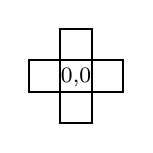
\begin{tikzpicture}[scale=0.8]
%\draw[step=0.5cm,lightgray,very thin] (0.5,0.5) grid (2,2);
\node at (1.25,1.22) {\textnormal{\footnotesize{0,0}}};
\draw[thick] (1,1) rectangle (1.5,1.5);
\draw[thick] (1.5,1) rectangle (2,1.5);
\draw[thick] (1,0.5) rectangle (1.5,1);
\draw[thick] (0.5,1) rectangle (1,1.5);
\draw[thick] (1,1.5) rectangle (1.5,2);
\end{tikzpicture} \\[0em]
(a)
\end{array}
\end{align*}
\end{minipage} $\rightarrow$ \begin{minipage}{0.43\linewidth}
\begin{align*}
\setlength{\arraycolsep}{0em}
\begin{array}{c}
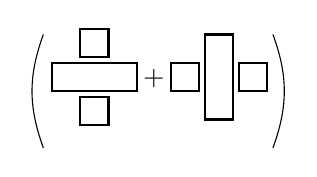
\begin{tikzpicture}[scale=0.72]
%\draw[step=0.5cm,lightgray,very thin] (0.5,0.5) grid (2,2);
%\node at (1.25,1.22) {\textnormal{\small{0,0}}};
\draw [black, thin] (0.35,0) to [round left paren ] (0.35,2);
\draw[thick] (0.5,1) rectangle (2,1.5);
\draw[thick] (1,0.40) rectangle (1.5,0.90);
\draw[thick] (1,1.60) rectangle (1.5,2.10);
\node at (2.3,1.22) {+};
\draw[thick] (3.8,1) rectangle (4.3,1.5);
\draw[thick] (2.6,1) rectangle (3.1,1.5);
\draw[thick] (3.2,0.5) rectangle (3.7,2);
\draw [black, thin] (4.4,0) to [round right paren ] (4.4,2);
\end{tikzpicture} \\[-0.5em] (b)
\end{array}
\end{align*}
\end{minipage}$\rightarrow$ \begin{minipage}{0.25\linewidth}
\begin{align*}
\setlength{\arraycolsep}{0em}
\begin{array}{c}
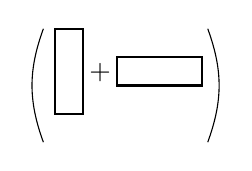
\begin{tikzpicture}[scale=0.72]
%\node at (1.25,1.22) {\textnormal{\small{0,0}}};
\draw [black, thin] (0.8,0) to [round left paren ] (0.8,2);
\draw[thick] (1,0.5) rectangle (1.5,2);
\node at (1.8,1.22) {+};
\draw[thick] (2.1,1) rectangle (3.6,1.5);
\draw [black, thin] (3.7,0) to [round right paren ] (3.7,2);
%\node at (2.75,1.22) {\textnormal{\small{0,0}}};
\end{tikzpicture} \\[-0.5em] (c)
\end{array}
\end{align*}
\end{minipage}
\caption{Illustration of grouping spans in
inference}
\label{fig:inference-steps-informal}
\vspace{-0.8em}
\end{figure}

\noindent
\textbf{1)\,} Compute all permutations on the column vectors in a span, \ie{},
  $[\vect{x}^L \vect{x}^U] \mapsto [\pi\vect{x}^L \, \pi\vect{x}^U]$
for a permutation $\pi$. For each permutation function $\pi^n_i$
(the $i$-th permutation for vectors of size $n$) we pair the
permutation function with the set of permuted spans so that
the spans can be un-permuted later.
%
\begin{equation*}
P(M) = \bigcup_{i \in n!} (\pi^n_{i} , \; \{[\pi^n_i
\vect{x}^L \; \pi^n_i\vect{x}^U] \, \mid \, [\vect{x}^L \; \vect{x}^U]
\leftarrow M\}
\end{equation*}
%
This corresponds to all rotations of the space, \eg{}:
%
\begin{align*}
P(M_0) =
\{&(\pi^2_1, \{ \stwo{0}{0}{0}{0},
\stwo{1}{0}{1}{0},
\stwo{-1}{0}{-1}{0},
\stwo{0}{1}{0}{1},
\stwo{0}{-1}{0}{-1} \})
\\
&(\pi^2_2, \{
 \stwo{0}{0}{0}{0},
 \stwo{0}{1}{0}{1},
 \stwo{0}{-1}{0}{-1},
 \stwo{1}{0}{1}{0},
 \stwo{-1}{0}{-1}{0}\})\}
\end{align*}
%
where $\pi^2_1$ is the identity permutation and $\pi^2_2$ is the
permutation that flips the order of the two elements in the
vectors.

\noindent
\textbf{2)\,} Sort each permutation set into a list, by the ordering:
\begin{equation*}
  \vect{x} \leq \vect{y} =
      \exists i \, . \; \vect{x}^L_{i} \leq \vect{y}^L_{i} \; \wedge \;
        (i = n \vee \vect{x}_{i+1:n} = \vect{y}_{i+1:n})
\end{equation*}
%
giving the sorting function $\textsf{sort}(M)$, \eg{}, $\textsf{sort}(P(M_0))$:
%%
\begin{align*}
\{&(\pi^2_1, [
\stwo{0}{-1}{0}{-1},
\stwo{-1}{0}{-1}{0},
\stwo{0}{0}{0}{0},
\stwo{1}{0}{1}{0},
\stwo{0}{1}{0}{1}] )
\\
&(\pi^2_2, [
\stwo{0}{-1}{0}{-1},
\stwo{-1}{0}{-1}{0},
\stwo{0}{0}{0}{0},
\stwo{1}{0}{1}{0},
\stwo{0}{1}{0}{1}])\}
\end{align*}
\noindent
\textbf{3)\,} Reduce each list pairwise by $\bullet$
(\Cref{def:span-coalesc}) to coalesce contiguous regions,
given by $\textsf{fold}\bullet$. For our example:
%
\begin{align*}
\{&(\pi^2_1, [
\stwo{0}{-1}{0}{-1},
\stwo{-1}{0}{1}{0},
\stwo{0}{1}{0}{1}
]), (\pi^2_2, \textit{same as for $\pi_1$})\}
\end{align*}
%
\textbf{4)\,} Un-permute and union together, \ie{},
%
\[
U(M) = \bigcup \{[\pi \vect{x}^L, \pi \vect{x}^U]
 \mid [\vect{x}^L, \vect{x}^U] \leftarrow S, (\pi, S) \leftarrow M\}
\]
For our example:
%
\begin{align*}
U(M) =
\{\stwo{0}{-1}{0}{-1},
\stwo{-1}{0}{1}{0},
\stwo{0}{1}{0}{1},
\stwo{-1}{0}{-1}{0},
\stwo{0}{-1}{0}{1},
\stwo{1}{0}{1}{0}\}
\end{align*}
%
\textbf{5)\,} Filter by the region containment predicate
$\containedin$; if any region is contained within another then remove the
  smaller, defined:
%
\begin{align*}
& \vect{x} \containedin \vect{y} = \vect{y}^L_1 \leq \vect{x}^L_1 \wedge \vect{x}^U_1 \leq \vect{y}^U_1
  \wedge (\vect{x}^L_{2:n}, \vect{x}^U_{2:n}) \containedin
  (\vect{y}^L_{2:n}, \vect{y}^U_{2:n})
\end{align*}
For our example this then yields the final result of:
\begin{align*}
\spanOp(M)
= \{\stwo{-1}{0}{1}{0} \stwo{0}{-1}{0}{1}\}
\end{align*}
since $\stwo{0}{1}{0}{1} \sqsubseteq \stwo{0}{-1}{0}{1}$
and $\stwo{1}{0}{1}{0} \sqsubseteq \stwo{-1}{0}{1}{0}$.
Applying \spanOp{} again yields the same
result for our example.%; the fixed point is reached.

\subsubsection{Step 4: Synthesise specifications from spans}
\label{sec:inf-step4}

\newcommand{\oplusbig}{\operatornamewithlimits{\term{\Large{$\oplus$}}}}
\newcommand{\odobig}{\operatornamewithlimits{\term{\Large{$\odot$}}}}
\newcommand{\bplus}{\operatornamewithlimits{\term{\Large{+}}}}
\newcommand{\tySum}[1]{#1^{\term{+}}}
\newcommand{\tyProd}[1]{#1^{\term{*}}}
\newcommand{\specDNF}{\textbf{spec}}

Abstract syntax trees of the specification language
are synthesised from the set $\spanOp(M)$ of coverings spans.
This conversion is defined in terms
of an algebra on \textit{spec} syntax in disjunctive-normal form
(which we denote \specDNF{}) and which is wrapped
in the $\textsf{Approx}$ type (see
\Cref{def:mult-and-approx}).  The algebra mirrors the shape
of the region operators $\term{+}$ and $\term{*}$ 
with binary operators $\oplus$ and $\odot$ on
$\mathsf{Approx}(\specDNF)$.
A function $\mathsf{toSpec}$ maps a dimension identifier
and a pair of lower and upper bound
values (one-dimensional) to a specification with a one-dimensional region.
%%
\begin{align*}
\mathsf{toSpec} & : \mathbb{N}_{>0} \rightarrow (\domainVal{} \times \domainVal{}) \rightarrow \mathsf{Approx}(\specDNF)
\end{align*}
%%
An entire span is converted into an $n$-dimensional
specification by applying $\mathsf{toSpec}$ to each
pair of lower and upper bounds in a span, per dimension, and multiplying these
specifications by $\odot$. The resulting specifications for
each span are then summed by $\oplus$:
\begin{equation*}
\textsf{spec}(M) =
\oplusbig\limits_{\vect{x} \in \spanOp(M)} \,
\odobig\limits_{i \in \{1, \ldots, n\}} \, \mathsf{toSpec} \; i \; (\vect{x}^L_i, \vect{x}^U_i)
\end{equation*}
We unpack the definitions of this algebra.

\begin{definition}[Specifications in DNF]
Let $r_1, ..., r_n$ range over elements of the \textit{region}
syntax (see \Cref{fig:syntax}).
The set \specDNF{} is a subset of syntax trees \textit{spec},
containing specifications in disjunctive normal form over regions
where the disjunct is \term{+} and the conjunct is \term{*}; 
 elements of \specDNF{} are of the form:
%%
$
(r^1_{1} \; \term{*} \ldots \term{*} \; r^1_n)\; \term{+} \; \ldots
\term{+} \; (r^m_1 \, \term{*} \; \ldots \term{*} \; r^m_p)
$.
%
%More formally, $\specDNF \subseteq (\textit{spec} \cup \{\epsilon\})$, defined:
%%%
%\begin{align*}
%\specDNF{} & ::= \tySum{\specDNF} \mid \epsilon \quad\;\;
%\tySum{\specDNF} ::= \tyProd{\specDNF} \; \term{+} \; \tySum{\specDNF} \mid
%  \tyProd{\specDNF} \\
%\tyProd{\specDNF} & ::= \textit{region} \; \term{*} \; \tyProd{\specDNF} \mid
%   \textit{region}
%\end{align*}
%%
In the following, $S, T$ range over elements of
\specDNF{} and $\tyProd{s}, \tyProd{t}$ range over conjuncts
 \eg{} $\tyProd{s} = r^1_{1} \; \term{*}
\ldots \term{*} \; r^1_n$.
\end{definition}

\newcommand{\exactR}{\mathsf{exact}\;}
\newcommand{\exact}[1]{\exactR(#1)}
\newcommand{\upperB}[1]{\mathsf{upper}\;(#1)}


\begin{figure}[t]
%\newcommand{\llower}{\vect{x}^L_i}
%\newcommand{\lupper}{\vect{x}^U_i}
\vspace{-0.7em}
\newcommand{\llower}{l}
\newcommand{\lupper}{u}
{\scalebox{0.95}{
\begin{minipage}{1\linewidth}
\begin{align*}
&\mathsf{toSpec} \; d \; (\llower, \lupper) = \\
&\hspace{-0.4em}\begin{cases}
%% POINT
\exact{\stenReflS{d}} & \llower = 0 \, \wedge \, \lupper = 0\\[0.02em]
%% FWD
\exact{\stenFwdS{\lupper}{d}}  & \llower = 0 \, \wedge \, \lupper > 0 \\[0.02em]
\exact{\stenFwdSR{\lupper}{d}{\irreflS}}\!\!\!\! & \llower = 1 \, \wedge \, \lupper > 0 \\[0.02em]
%% BWD
\exact{\stenBwdS{|\llower|}{d}}  & \llower < 0 \, \wedge \, \lupper = 0 \\[0.02em]
\exact{\stenBwdSR{|\llower|}{d}{\irreflS}}\!\!\!\! & \llower < 0 \, \wedge \, \lupper = -1 \\[0.02em]
%% CEN
\exact{\stenCenS{\lupper}{d}}& \!\!\!\llower < 0 \wedge \lupper > 0 \wedge |\llower| = \lupper \\[0.02em]
\exactR(\stenBwdS{|\llower|}{d} & \!\!\!\llower < 0 \wedge \lupper > 0  \wedge |\llower| \neq \lupper \\
\qquad\qquad \texttt{+} \, \stenFwdS{\lupper}{d}) & \\[0.02em]
% BOUND
\upperB{\stenFwdS{\lupper}{d}} & \llower > 1 \\[0.02em]
\upperB{\stenBwdS{|\llower|}{d}} \quad & \llower < (-1)
 \\[0.02em]
% ABSOLUTE REP
\exact{\epsilon} & \llower = \infty \, \vee \, \lupper = \infty
  \end{cases}
\end{align*}
\end{minipage}
}}
\caption{\textsf{toSpec} constructor of $\mathsf{Approx}(\specDNF)$ values.}
\label{fig:to-spec}
\vspace{-0.8em}
\end{figure}

\begin{definition} The $\mathsf{toSpec}$ constructor is defined
in \Cref{fig:to-spec}, where the lower and upper bounds
determine region constants; $\mathsf{toSpec} \, d \, (l, u)$ is defined
 if $l$ less than or equal to $u$.

Positive lower and upper bound yield \term{forward} regions, and
negative lower and upper bounds yield \term{backward} regions.
The \texttt{nonpointed} attribute (abbreviated \term{np})
is present when the lower bound is at $1$ or $-1$. 
In the sixth-case, where the lower bound
is negative and the upper bound is positive and they have the same
magnitude, then a \texttt{centered} region is constructed with
the depth as the common magnitude. If the magnitudes are not the same
(seventh case) then separated \texttt{forward} and \texttt{backward}
regions are summed, with their corresponding depths.
If the lower bound is greater than 1
(which implies the upper bound is greater than 1 too) then
this represents a region that is not at the origin (or next to) the
origin and thus cannot be represented in the specification language.
Thus, an upper bound is produced showing the maximum extent
of the region. The penultimate case is the dual, when the lower bound is less
than $-1$, giving an upper bound on a \texttt{backward} specification.
\end{definition}

\begin{definition} The $\odot$ operation on $\textsf{Approx}(\specDNF{})$
  is defined in terms of the intermediate operator $\hat{\odot}$ on
  \specDNF{}, defined:
%%
\begin{align*}
S \,\hat{\odot}\, \epsilon = S \quad
\epsilon \,\hat{\odot}\, S = S \qquad
S \,\hat{\odot}\, T = \bplus_{(\tyProd{s}, \tyProd{t}) \in (S \times
   T)} (\tyProd{s} \; \term{*} \; \tyProd{t})
\end{align*}
%%
That is, the $\hat{\odot}$ product of two specifications $S$ and $T$ in DNF form
is the $\term{+}$ sum of all pairwise $\term{*}$ products for every
pair of $\tyProd{spec}$ drawn from $S$ and $T$. The result
is indeed in DNF-form, where $\hat{\odot}$ is essentially applying
 the \trule{\textsc{dist}} rule of the equational theory. The operation is
commutative and associative, and sound with respect to our
model (see \Cref{lem:alg-soundness} below).
The $\hat{\odot}$ operation is then lifted to all combinations of
\textsf{Approx} for $\odot$:
\begin{align*}
\textsf{lower}(S) \odot \textsf{exact}(T) = \; &
       %\textsf{exact}(T) \odot \textsf{lower}(S) = \;
       \textsf{both} \, (S \hat{\odot} T, \; T) \\
\textsf{upper}(S) \odot \textsf{exact}(T) = \; &
       %\textsf{exact}(T) \odot \textsf{upper}(S) =
       \textsf{both} \, (T, \; S \hat{\odot} T) \\
\textsf{lower}(S) \odot \textsf{both}(T_l,T_u) = \; &
        %\textsf{both}(T_l,T_u) \odot \textsf{lower}(S) = \;
        \textsf{both} \, (S \hat{\odot} T_l, \; T_u) \\
\textsf{upper}(S) \odot \textsf{both}(T_l,T_u) = \; & \textsf{both} \,
                                                      (T_l, \; S \hat{\odot} T_u) \\
\textsf{both}(S_l,S_u) \odot
\textsf{both}(T_l,T_u)  = \; & \textsf{both} (S_l \hat{\odot} T_l, \; S_u
                         \hat{\odot} T_u) \\
\textit{inj}(S) \odot \textit{inj}(T) = \; & \textit{inj}(S
                                              \hat{\odot} T)
\end{align*}
where in the last case $\textit{inj}$ corresponds to the unary
injections of \textsf{Approx}. For brevity we omit the cases where the arguments above are flipped
as $\odot$ is commutative.
\end{definition}

\begin{definition}The $\oplus$ operation on $\textsf{Approx}(\specDNF)$
is defined similarly to $\odot$, with the intermediate $\hat{\oplus}$ on
$\specDNF$:
%%
\begin{equation*}
S \,\hat{\oplus}\, \epsilon = S \quad
\epsilon \,\hat{\oplus}\, S = S \quad
S \, \hat{\oplus} \, T = S \, \term{+} \, T
\end{equation*}
%%
Thus, if neither specification is empty, their $\hat{\oplus}$ is just
the syntactic sum $\term{+}$. Then $\oplus$ is the lifting of
$\hat{\oplus}$ to \textsf{Approx} with the shape as $\odot$ in the previous
definition.
\end{definition}

\begin{lemma}%[$\hat{\odot}$, $\hat{\oplus}$ soundness]
$\forall S,
  T \in \specDNF$ where $S\!\neq \epsilon \wedge T\!\neq \epsilon$:
\begin{align*}
\interp{S \; \hat{\odot} \; T}_n = \interp{S}_n \otimes \interp{T}_n
  \qquad
\interp{S \; \hat{\oplus} \; T}_n = \interp{S}_n \cup \interp{T}_n
\end{align*}
\label{lem:alg-soundness}
\vspace{-2em}
\end{lemma}
%
\noindent
Thus our model validates the specification synthesis process which concludes the
inference procedure. For our example, we infer and then synthesise the
5-point specification:
%%
\begin{minted}[linenos=false]{fortran}
!= stencil centered(depth=1, dim=1)*pointed(dim=2) + centered(depth=1, dim=2)*pointed(dim=1):: a
\end{minted}
%%

\section{Evaluation}
\label{sec:evaluation}

%We have processed nearly one million lines of Fortran code using our
%CamFort tool and examined the output to determine how useful
%and applicable it may be. Our corpus of Fortran code is collected from
%many computational science projects for which we believe our tool will
%be potentially helpful.

% Corpus details
% specfem3d ``simulates acoustic (fluid), elastic (solid), coupled
% acoustic/elastic, poroelastic or seismic wave propagation in any
% type of conforming mesh of hexahedra (structured or not).''
% https://github.com/geodynamics/specfem3d

% arpack-ng - Fortran 77 routines designed to solve large scaled
% eigenvalue problems - https://github.com/opencollab/arpack-ng

We first examined how frequently stencil computations occur in our
corpus of Fortran code. This was carried out by running CamFort in
whole-code-base inference mode. We parsed 959,427 lines of Fortran
code and found that 10\% (97,439) of statements have a left-hand side
is an array subscript on neighbourhood indices. This supports the idea
that stencil-like computations are common in scientific code. 

We would not expect to infer a stencil for each of these statements
because our stencil language places significant restrictions on the
types of array-subscript-statements that we will class as a
stencil. In fact, CamFort was able to infer a stencil from 30\% of
these statements. A single statement can produce multiple stencils and
we ended up with 60,525 stencils. This shows that we can still express
a large number of stencil uses within our high-level abstraction.

There were a variety of reasons why we did not infer a
stencil from every potential statement: \\
\noindent 
1) \textbf{Non-subset induction variables} occur when the
induction variables on the RHS are not a subset of those in the LHS. These
cases are not stencils by our definition. The degenerate case of this
is to have only constant indices on the LHS. We see lots of examples
of this in loops as accumulators \eg{} computing the sum over an array; \\
\noindent
2) \textbf{Derived induction variables} where the
indexing variable (\mintinline{fortran}{x}) is derived from an
induction variable (\mintinline{fortran}{i}) as in
\mintinline{fortran}{x = len - i};  \\
\noindent
3) \textbf{Inconsistent induction dimensions} occur when
an induction variable is used to specify more than one array dimension
on the RHS or multiple induction variables are used for the same
dimension on the RHS. These are common in matrix operations such as
LU-decomposition with assignments such as
\mintinline{fortran}{a(l) = a(l) - a(m) * b(l, m)}.


%    numStencilSpecs: 60525
% 4338 files, linesTotal: 1357377, linesParsed: 959427
% Number of stencils (tickAssign) / number of loops
% Percentage of a code base that is taken up by stencils
%Out of 1.35 million lines of code that we fed into our program, and
%the 959,427 lines that we were able to parse, we identified 60,525
%cases that fit our criteria for stencil specification.

%\paragraph{Hypothesis 2: Most stencil computations
%have a regular pattern which can be captured with a simple
%language of contiguous regions}

% Number of stencils we give a spec to (where a spec declaration to n
% variables is counted n times) as percentage of number of stencils

    % tickAssign: 97439
    % tickAssignSuccess: 29402 % <- number of times tickAssign is accompanied by a successful stencil inference
                               % counts only by +1 each time that tickAssign finds a stencil

%In the analysed body of code we found that we were able to deduce
%some form of stencil specification from approximately 30\% of the
%potential stencils examined.


%
%\subsection{Analysing the design of our specifications}

% 1. How may are just reflexive and how many some reflexive
% justReflexive: 55504
% someReflexive: 15823

The vast majority of stencils we found were relatively simple but we
found significant numbers of more complex shapes. We grouped common
patterns in to categories which we describe below.

\textbf{All pointed} 55,504 of the stencils we found involved 
only pointed regions. 39,681 of these were pointed in all
dimensions. Common examples of this were pointwise transformations on
data (such as scaling).

\textbf{Single-action} specifications consist of no more than one 
forward, backward, or centered region and can be combined with any
number of pointed regions. We identified 4,837 single-action
specifications, of which 1,532 were single-action with a
\texttt{nonpointed} modifier.

\textbf{Multi-action} specifications consist of at least two uses 
of forward, backward, or centered regions, and can be combined with
any number of pointed regions. We identified 156 multi-action
specifications out of which 146 had regions combined only with
$\term{*}$.

\textbf{Bounded} specifications were fairly unusual, with only 157
\texttt{atMost} and 36 \texttt{atLeast}, the latter of which were
always also bounded on both sides.

\begin{figure}[t]\begin{minted}[fontsize=\scriptsize,breakindent=0em,linenos=false,xleftmargin=0em,breakafter=)]{fortran}
!=stencil readOnce,(forward(depth=1,dim=3,nonpointed))*(backward(depth=1,dim=1))*(backward(depth=1,dim=2))+(forward(depth=1,dim=3))*(backward(depth=1,dim=1))*(pointed(dim=2))+(forward(depth=1,dim=3))*(backward(depth=1,dim=1,nonpointed))*(backward(depth=1,dim=2,nonpointed))+(forward(depth=1,dim=3))*(backward(depth=1,dim=2))*(pointed(dim=1))+(backward(depth=1,dim=1))*(backward(depth=1,dim=2,nonpointed))*(pointed(dim=3))+(backward(depth=1,dim=1,nonpointed))*(backward(depth=1,dim=2))*(pointed(dim=3))::x
\end{minted}
\caption{A complex specification inferred from
  \textbf{Unified Model}\label{fig:smagorinsky}}
\vspace{-1em}
\end{figure}

The single- and multi-action classes represent more complex stencils
with a real possibility for programmer error. For example, the Unified
Model has an implementation of the Smagorinsky subgrid-scale model for
calculating turbulence on which our inference yields 39 specs from 340
lines of code. This is an impressive reduction given
the complexity of the algorithm.  We show one example in
Figure~\cref{fig:smagorinsky}. This specifies the access pattern to
a 3-dimensional array (which we have renamed to be called
\texttt{x}). The array is accessed 8 times in the computation.

\subsection{Detecting errors in the 2-D Jacobi iteration}

One common example of a stencil computation is two-dimensional
Jacobi iteration that repeatedly goes through each cell in a matrix
and computes the average value of the four adjacent cells. The kernel
can be expressed in a line of Fortran code:
\begin{minted}{fortran}
  a(i,j) = (a(i-1,j)+a(i+1,j)+a(i,j+1)+a(i,j-1))/4
\end{minted}
and CamFort is able to infer a precise specification for this:
\begin{minted}[breakafter=+:,breakindent=-0.6em,breaksymbolsep=0.4em,linenos=false,xleftmargin=-0.5em]{fortran}
  != stencil pointed(dim=1)*centered(depth=1,dim=2,nonpointed)+pointed(dim=2)*centered(depth=1,dim=1,nonpointed)::a
\end{minted}

We examined whether programmer errors would be detected by replacing
the array index offsets with $-1$, $0$, or $1$ and running our
verification algorithm. Camfort correctly reported a verification
failure in each of 6,537 permutations corresponding to an error.  We
note that the iteration is computing the average of four adjacent
cells so $24$ ($4!$) of the possible array index pertubations do not
correspond to a programming error.


% /um/trunk/src/atmosphere/diffusion_and_filtering/turb_smagorinsky.F90
% Tried introducing indexing errors replacing one of the indices of cx_rho_instance with -1,0,+1
% 42 cases were caught
% 6 cases were not caught


% (/ 55504.0 60525) = 91.7%
% (/ 15823.0 60525) = 26.1%
% 91.7\% of the specifications involved only reflexive regions. 26.1\%


% 2. Break down of "interesting specifications" (contain more than
% just reflexive)
%   - Single-action, histogram on depths
%   - Single-action + irreflexives, histogram on depths

% singleAction: 4837
% singleActionIrr: 1532

%   - Multi-action combined only by *
%   - Multi-action combined also by +, histogram of tree depths

    % multiAction: 156
    % multiActionMulOnly: 146




%   - Bounded specs (how many lower, upper, or both)


    % atLeast: 36
    % atMost: 157
    % boundedBoth: 36



% Present not just percentages but concrete numbers

\section{Related work and conclusions}
\label{sec:discussion}

Various deductive verification tools can express array indexing
in their specifications, \eg{}, ACSL of \citet{baudin2008acsl}
for C (see \eg{}~\citet[Example 3.4.1]{burghardt2010acsl}). Thus, a specification
can be given for a stencil computation, 
however, such a specification would exactly replicate the fine-grained
indexing seen in the code and would simply be prone to low-level input
errors. Our approach is much more abstract-- it does
not aim to reify indexing in the specification, but is novel
in that it instead
provides abstract spatial descriptions which capture a large number
of common patterns.

\citet{kamil2016verified} propose \emph{verified lifting} to extract a
functionally-complete mathematical representation of low-level, and
potentially optimised, stencils in Fortran code. This extracted
predicate representation of a stencil is used to generate code
for the \textsf{Halide} high-performance
compiler~\citep{ragan2013halide}. Thus their approach must capture the
full meaning of a stencil computation which requires significant
program analysis. For example, they report that some degenerate
stencil kernels take up to 17 hours to analyse and others require
programmer intervention for correct invariants to be inferred.

% ACR-I think we could skip this in the interests of space
%This led them to develop \textsf{STNG}, a loop invariant and postcondition
%finder through syntax-guided synthesis. Using this approach they restrict the
%search space of postconditions to predicates of a certain form, one that is
%compatible with \textsf{Halide}. They then look at concrete loop iterations and
%form an hypothesis about the invariant, which is later confirmed or put back
%into the system using a SMT solver.

Our approach differs significantly. Rather than 
full representation of stencils, we focus on specifying
just the spatial behaviour in a lightweight way.
Thus, it suffices for us to perform a comparatively
simple data-flow analysis which is efficient, scales linearly with
code size, and does not require any user intervention.
Whilst we do not perform deep semantic analysis of stencils,
 the analysis part of our
approach can be made arbitrarily more sophisticated independent of the rest of
the work.
% Hence, we do not require SMT solving or search of loop invariants. It
%suffices to do comparatively simple data-flow analysis.
%Since CamFort mostly does
%syntactic analysis, the inference procedure terminates quickly and
%never requires programmer intervention. 
%The downside of our
%approach is that if optimisation causes the stencil computation to be heavily
%obfuscated, \textsf{STNG} would capture the access behaviour better.
%
Furthermore, Kamil \emph{et al.} do not provide a user-visible
syntactic representation of their specifications, and they do
not use their specifications for verification, \eg{}, to future-proof
the code against later changes. Even if they were to provide a
syntactic representation, for complex stencils such as Navier-Stokes
from \cref{sec:intro}, it would be as verbose as the code itself,
making it difficult for programmer to understand the overall shape of
the indexing behaviour.

% GPGPU
Our work has some similarities with efforts to verify kernels
written for General-Purpose Graphics Processing Unit (GPGPU)
programming, such as in \citet{Blom:2014:SoCP}. %Stencils are a form of
%kernel, and GPGPU programming can be viewed as a massively parallel
%method of transforming a large matrix. 
However, their focus is
mainly on the synchronisation of kernels and the avoidance of
data races, while we are interested in correctness 
embedded within a more typical general-purpose programming
language. %Other work on GPGPU computation, such as
%\citet{Zhang:2012:CGO}, has focused primarily on generating
%optimised code based on relatively simple specifications: to
%provide performance while keeping the programmer's effort within
%reason.

% Sketching Stencils
\citet{Solar-Lezama:2007:PLDI} give specifications of stencils using
unoptimised ``reference'' stencils, coupled with partial
implementations which are then completed by a code
generation tool. %These kinds of specifications are just simple
%implementations, so this tool is useful for hand-written, optimised
%stencils. 
The primary purpose of this tool is optimisation rather than
correctness, and the language of specification is much different and
more elaborate than in our approach.

% Pochoir
\citet{Tang:2011:SPAA} define a specification language for writing
stencils embedded in C++ (with Cilk extensions) that are then compiled
into fast parallel programs based on trapezoidal decompositions with
hyperspace cuts. The Pochoir specification language is used for
describing the kernel, boundary conditions and shape of the
stencil. Programs are first compiled in C++ with a template library
that checks whether the annotations are used correctly, and then a
Pochoir preprocessor may be applied to generate the high-performance
parallel versions using Cilk.  Pochoir
is aimed primarily at assisting programmers who may be reluctant to
implement the high-performance tricky cache-oblivious
``hypertrapezoidal'' algorithms for stencils. 
%that are significantly faster than the typical looping implementations
%of stencil computations.
Like much of the related work, the main goal 
is optimisation rather than verifying program correctness.

By contrast, the work of \citet{Abe:2013:IPDPSW} has looked at the
correctness problem explicitly by bringing a form of model-checking to
verify certain stencil computations. This is in the context of
decomposing stencils for parallel computation on multiple processors
 in partitioned global address
space languages. %These are scenarios where an array is divided into
%subarrays on multiple processors but each has the ability to access
%the others' memory. The authors avoid the state explosion dilemma of
%model-checking by relying upon the fact that accesses to the
%``boundary elements'' will require a different method by virtue of the
%non-locality of that memory. Since this access is performed in a
%different manner, those can be identified automatically by static
%analysis. To achieve this, 
Abe \emph{et al.} provide a new language to
be used for writing stencil computations. Much of the specification
effort goes towards describing the nuts and bolts of distributing the
computation over multiple processors. The code for the stencil kernel
is generated from a relatively high-level specification. 
In contrast, we are interested in integrating directly
into existing, legacy codebases and established languages, bringing
the benefits of verification more easily to scientific computing.%such as
%older versions of Fortran.% We infer stencil specifications from
%Fortran code and check annotations on stencil computations within
%Fortran code.

\paragraph{Concluding remarks}

There is an increasing awareness of the need for verification
techniques in
science~\cite{post2005computational,oberkampf2010verification,orchard2014computational}.
Our specification language is an approach in this direction, providing
a system of lightweight, high-level specification for numerical code.
As opposed to existing approaches our language takes inspiration from
the numerical literature and provides a concise, abstract description
of the stencil.

We evaluated our approach on top of CamFort, an open-source analysis
tool for Fortran programs, running the inference process over a corpus
of a million lines of Fortran code. We showed that our language is
capable of capturing many real-world uses of stencils and showed in a
case-study that it will detect (simulated) programmer errors.

Our definition of a stencil computation meant that we generated no
specification for a large number of iterated array accesses in the
corpus, such as stencils that incorporates reductions. For
future work, we will be looking into expanding the flexibility of 
our analysis to include these examples. 

\bibliography{references}

\end{document}

%%  LocalWords:  refactoring affine parameterised nonpointed atMost
%%  LocalWords:  centered readOnce atLeast discretisation Equational
%%  LocalWords:  equational disjunction denotational dimensionality
%%  LocalWords:  interprocedural Fortran CamFort preprocessor
%%  LocalWords:  committers
